% ============================================================
%  Guía de estudio — Arquitectura de Redes I (PEI 1: Temas 1 y 2)
%  Compilar con:  pdflatex resumen_PEI1_AR1.tex  (dos pasadas)
% ============================================================
\documentclass[11pt,a4paper]{article}

\usepackage[utf8]{inputenc}
\usepackage[T1]{fontenc}
\usepackage{mathpazo}
\usepackage[scaled=.92]{helvet}
\IfFileExists{spanish.ldf}{%
  \usepackage[spanish,es-noshorthands]{babel}\decimalpoint
}{%
  \renewcommand{\contentsname}{Índice}\renewcommand{\tablename}{Tabla}\renewcommand{\figurename}{Figura}%
}
\usepackage[margin=2.2cm,top=2.6cm,bottom=2.4cm]{geometry}
\usepackage[table]{xcolor}
\usepackage{amsmath,amssymb}
\usepackage{booktabs,array,tabularx,longtable}
\usepackage{enumitem}
\usepackage{microtype}
\usepackage{fancyhdr}
\usepackage{titlesec}
\usepackage{tikz}
\usetikzlibrary{arrows.meta,positioning,calc,shapes.geometric}
\usepackage[most]{tcolorbox}
\usepackage{listings}
\usepackage[colorlinks=true,linkcolor=uahblue,urlcolor=uahblue]{hyperref}

% ---------- Colores ----------
\definecolor{uahblue}{RGB}{0,86,164}
\definecolor{uahsand}{RGB}{234,224,200}
\definecolor{okgreen}{RGB}{30,120,70}
\definecolor{warnred}{RGB}{170,40,40}
\definecolor{codebg}{RGB}{248,248,246}
\definecolor{codegray}{RGB}{110,110,110}

% ---------- Títulos ----------
\titleformat{\section}{\Large\sffamily\bfseries\color{uahblue}}{\thesection.}{0.6em}{}[\vspace{-0.5em}\color{uahblue}\titlerule]
\titleformat{\subsection}{\large\sffamily\bfseries\color{uahblue}}{\thesubsection}{0.6em}{}
\titleformat{\subsubsection}{\normalsize\sffamily\bfseries\color{uahblue!80!black}}{}{0em}{}
\titlespacing*{\section}{0pt}{1.6em}{0.9em}
\titlespacing*{\subsection}{0pt}{1.2em}{0.5em}
\titlespacing*{\subsubsection}{0pt}{1em}{0.3em}

% ---------- Cabecera y pie ----------
\pagestyle{fancy}
\fancyhf{}
\renewcommand{\headrule}{\hbox to\headwidth{\color{uahblue}\leaders\hrule height 0.4pt\hfill}}
\lhead{\small\sffamily\color{uahblue}\textbf{Arquitectura de Redes I}}
\rhead{\small\sffamily\color{gray}Guía de estudio PEI\,1 --- Temas 1 y 2}
\cfoot{\small\thepage}
\setlength{\headheight}{22pt}

\setlist{itemsep=2pt,topsep=4pt}
\setlength{\parindent}{0pt}
\setlength{\parskip}{5pt}
\renewcommand{\arraystretch}{1.25}

% ---------- Cajas ----------
\newtcolorbox{definicion}[1][]{colback=uahblue!6,colframe=uahblue,boxrule=0.6pt,arc=2pt,
  left=8pt,right=8pt,top=5pt,bottom=5pt,title={#1},fonttitle=\sffamily\bfseries,breakable}
\newtcolorbox{formula}[1][]{colback=okgreen!6,colframe=okgreen,boxrule=0.6pt,arc=2pt,
  left=8pt,right=8pt,top=5pt,bottom=5pt,title={#1},fonttitle=\sffamily\bfseries,breakable}
\newtcolorbox{ojo}[1][]{colback=warnred!5,colframe=warnred,boxrule=0.6pt,arc=2pt,
  left=8pt,right=8pt,top=5pt,bottom=5pt,title={#1},fonttitle=\sffamily\bfseries,breakable}
\newtcolorbox{nota}[1][]{colback=uahsand!45,colframe=uahsand!90!black,coltitle=black,boxrule=0.6pt,arc=2pt,
  left=8pt,right=8pt,top=5pt,bottom=5pt,title={#1},fonttitle=\sffamily\bfseries,breakable}

\newcolumntype{L}[1]{>{\raggedright\arraybackslash}p{#1}}
\newcommand{\hd}[1]{\cellcolor{uahblue}\textcolor{white}{\textbf{#1}}}
\newcommand{\en}[1]{\emph{(#1)}}

% ---------- Código ----------
\lstset{
  basicstyle=\ttfamily\small,
  backgroundcolor=\color{codebg},
  frame=single,
  rulecolor=\color{uahblue!40},
  keywordstyle=\color{uahblue}\bfseries,
  commentstyle=\color{codegray}\itshape,
  stringstyle=\color{okgreen!70!black},
  showstringspaces=false,
  breaklines=true,
  columns=fixed,basewidth=0.5em,
  keepspaces=true,
  aboveskip=6pt,belowskip=6pt,
  xleftmargin=2pt,xrightmargin=2pt
}
\lstdefinelanguage{pyr}{
  morekeywords={from,import,while,True,input,print,def,with,as,if,else},
  sensitive=true, morecomment=[l]{\#}, morestring=[b]', morestring=[b]"
}
\lstdefinelanguage{httpmsg}{}

\begin{document}

% ============================================================
%  CABECERA DEL DOCUMENTO
% ============================================================
\begin{tcolorbox}[colback=uahblue,colframe=uahblue,arc=0pt,top=14pt,bottom=14pt,left=14pt,right=14pt]
{\sffamily\Huge\bfseries\color{white}Guía de estudio}\\[4pt]
{\sffamily\Large\color{white}Arquitectura de Redes I --- PEI\,1}\\[4pt]
{\sffamily\color{white!85!uahblue}Tema 1: Arquitecturas de red \quad|\quad Tema 2: Protocolos de la capa de aplicación}
\end{tcolorbox}

\begin{definicion}[Qué entra en la PEI\,1 (guía docente 2026/27)]
La PEI\,1 se hace hacia mitad de cuatrimestre, pesa el \textbf{30\,\%} y cubre los \textbf{Temas 1 y 2}, con teoría y problemas (cuestiones de desarrollo o test y ejercicios). Resultados de aprendizaje evaluados: RA1--RA8, RA10 y RA11.
\vspace{2pt}
\begin{tabularx}{\linewidth}{@{}L{6.4cm}X@{}}
\toprule
\hd{Contenido oficial} & \hd{Dónde está en esta guía} \\
\midrule
T1: elementos de red, protocolos, retardos, lógica de redes, OSI, TCP/IP & Sección 1 (RA1--RA6) \\
T2: aplicaciones distribuidas, cliente/servidor, HTTP, DNS, sockets & Sección 2 (RA7, RA8, RA10) \\
Cálculo de parámetros de eficiencia & Subsecciones 1.2, 1.4 y 1.8, ejercicios y hoja de fórmulas (RA6) \\
Exámenes de años anteriores (PEI\,1, EE, PP) & Sección 4: problemas resueltos y respuestas de test; DNS y HTTP en 2.3 y 2.4 \\
\bottomrule
\end{tabularx}

Formato visto en exámenes anteriores: test de 10 preguntas (5 puntos; acierto $+0{,}5$, fallo $-0{,}1$, blanco $0$) y dos problemas (de 2 y 3 puntos). FTP, correo (SMTP, POP3, IMAP) y BitTorrent no figuran en los contenidos oficiales (solo web y DNS), pero sí en las diapositivas: están resumidos en 2.5 por si salen en el test.
\end{definicion}

\begin{definicion}[Cómo usar esta guía]
Resumen de los \textbf{Temas 1 y 2} (PEI\,1, 30\,\% de la nota) basado en el resumen previo, revisado y ampliado con \emph{Redes de computadoras: un enfoque descendente} (Kurose \& Ross, 7.\textsuperscript{a} ed.).
\begin{itemize}[leftmargin=1.2em]
  \item Las cajas \textbf{verdes} contienen fórmulas.
  \item Las cajas \textbf{rojas} marcan errores frecuentes de examen.
  \item Al final hay \textbf{ejercicios resueltos}, \textbf{problemas de exámenes anteriores} y una \textbf{hoja de fórmulas}.
  \item La última sección lista las \textbf{correcciones} hechas respecto al resumen original.
\end{itemize}
\end{definicion}

\tableofcontents
\newpage

% ============================================================
%  TEMA 1
% ============================================================
\section{Tema 1: Arquitecturas de red}

% ------------------------------------------------------------
\subsection{Elementos de una red}

Internet es una red de redes formada por miles de millones de dispositivos, \emph{enlaces} y \emph{conmutadores de paquetes}. Se describe en tres partes:

\begin{itemize}
  \item \textbf{Borde de la red.} Sistemas finales (\emph{hosts}) que ejecutan aplicaciones. Se agrupan en \textbf{clientes} (PC, móviles, dispositivos IoT, que inician peticiones) y \textbf{servidores} (máquinas en centros de datos que atienden peticiones y distribuyen contenido).
  \item \textbf{Redes de acceso.} Enlaces que conectan un sistema final con el primer router (\emph{edge router}).
  \item \textbf{Núcleo de la red.} Malla de routers interconectados con enlaces de alta capacidad (fibra óptica terrestre y submarina) que transporta los datos de la red de acceso de origen a la de destino.
\end{itemize}

\subsubsection{Tecnologías de acceso}

\begin{tabularx}{\textwidth}{@{}L{2.6cm}L{3.3cm}X@{}}
\toprule
\hd{Tecnología} & \hd{Medio} & \hd{Características clave} \\
\midrule
\textbf{FTTH} \en{fibra hasta el hogar} & Fibra óptica & Fibra hasta la vivienda. Arquitectura típica PON (óptica pasiva): un divisor óptico reparte la fibra entre varios hogares. GPON es asimétrica (en torno a 2{,}5 Gbps de bajada y 1{,}25 Gbps de subida); XGS-PON ofrece 10 Gbps simétricos. \\
\textbf{HFC} \en{híbrido fibra-coaxial} & Fibra hasta el nodo de zona y coaxial hasta el hogar & Medio \textbf{compartido} entre los usuarios del vecindario. Usa el estándar \textbf{DOCSIS}. Canales de bajada y subida \textbf{asimétricos}. \\
\textbf{DSL} & Par trenzado de cobre de la red telefónica & Línea \textbf{dedicada} hasta la central. Con \textbf{FDM} se divide en tres bandas: telefonía bidireccional (hasta 4~kHz), subida (4--50~kHz) y bajada (50~kHz--1~MHz). La velocidad cae con la distancia a la central. \\
\textbf{Ethernet} (IEEE 802.3) & Par trenzado (UTP Cat\,5e/6/7) con conectores RJ-45; también fibra & Acceso LAN en empresas, universidades y hogares mediante \emph{switches}. Velocidades de 100~Mbps, 1~Gbps, 10~Gbps o más. \\
\textbf{Wi-Fi} (IEEE 802.11) & Radio, bandas sin licencia (2{,}4, 5 y 6~GHz) & Acceso inalámbrico local mediante un punto de acceso. Usa acceso múltiple (CSMA/CA) para compartir el canal. \\
\textbf{Celular} (4G LTE, 5G NR) & Radio, espectro con licencia & Acceso inalámbrico de área extensa mediante estaciones base (eNodeB / gNodeB), con soporte de movilidad. \\
\bottomrule
\end{tabularx}

\subsubsection{Medios físicos}

\begin{tabularx}{\textwidth}{@{}L{3.2cm}X@{}}
\toprule
\hd{Medio} & \hd{Observaciones} \\
\midrule
Par trenzado & Barato y muy extendido. Velocidades de 100~Mbps a 10~Gbps según categoría y longitud. \\
Cable coaxial & Dos conductores concéntricos. Admite medio compartido y velocidades altas; base de HFC. \\
Fibra óptica & Pulsos de luz. Muy alta velocidad (decenas o cientos de Gbps), baja atenuación e inmunidad al ruido electromagnético. Es el medio del núcleo. \\
Radio terrestre & Sin cableado físico; sensible a interferencias, obstáculos y multitrayecto. \\
Satélite & Geoestacionario (a unos 36\,000~km, con retardo de propagación en torno a 280~ms) o de órbita baja, con retardo mucho menor. \\
\bottomrule
\end{tabularx}

\subsubsection{Clasificación de las redes}

\begin{tabularx}{\textwidth}{@{}L{3.6cm}X@{}}
\toprule
\hd{Criterio} & \hd{Categorías} \\
\midrule
Topología & \textbf{Malla} (cada nodo conectado con varios otros; muy robusta y costosa), \textbf{estrella} (todos los nodos a un nodo central; un fallo central deja la red incomunicada), \textbf{árbol} (jerarquía de estrellas). \\
Alcance geográfico & \textbf{LAN} (edificio o campus), \textbf{MAN} (ciudad o área metropolitana), \textbf{WAN} (país o continente). \\
Cercanía al usuario & \textbf{Acceso} (hasta el usuario), \textbf{agregación} (concentra el tráfico de muchos accesos), \textbf{núcleo} (transporte troncal). \\
Medio con el usuario & \textbf{Cableada} (cobre, fibra) o \textbf{radio} (Wi-Fi, celular, satélite). \\
Movilidad & \textbf{Fija} o \textbf{móvil}. \\
Tipo de servicio & Datos, voz, vídeo, servicios interactivos y multimedia. \\
\bottomrule
\end{tabularx}

\subsubsection{Red del hogar}

Pregunta típica de examen: dibujar el esquema de una red doméstica con acceso a Internet, indicando la función de cada elemento y cómo se interconecta.

\begin{center}
\begin{tikzpicture}[font=\small\sffamily,
  n/.style={draw=uahblue,fill=uahblue!8,rounded corners=2pt,minimum height=0.8cm,minimum width=2.1cm,align=center},
  s/.style={draw=uahblue,fill=uahsand!60,rounded corners=2pt,minimum height=0.8cm,minimum width=2.1cm,align=center},
  l/.style={thick,uahblue},
  lab/.style={font=\scriptsize,fill=white,inner sep=1pt}]
  \node[s] (isp) at (0,0) {ISP / Internet};
  \node[n] (ont) at (3.6,0) {ONT / módem\\[-2pt]\scriptsize (fibra, cable, DSL)};
  \node[n] (rt) at (7.5,0) {Router\\[-2pt]\scriptsize NAT, DHCP, firewall};
  \node[n] (sw) at (10.9,1.2) {Switch\\[-2pt]\scriptsize Ethernet};
  \node[n] (ap) at (10.9,-1.2) {Punto de acceso\\[-2pt]\scriptsize Wi-Fi};
  \node[n] (pc) at (13.9,1.7) {PC};
  \node[n] (tv) at (13.9,0.7) {Smart TV};
  \node[n] (mv) at (13.9,-0.7) {Móvil};
  \node[n] (iot) at (13.9,-1.7) {Dispositivo IoT};
  \draw[l] (isp)--(ont) node[midway,above,lab]{acceso};
  \draw[l] (ont)--(rt) node[midway,above,lab]{Ethernet};
  \draw[l] (rt)--(sw); \draw[l] (rt)--(ap);
  \draw[l] (sw)--(pc); \draw[l] (sw)--(tv);
  \draw[l,dashed] (ap)--(mv); \draw[l,dashed] (ap)--(iot);
\end{tikzpicture}
\end{center}

\begin{tabularx}{\textwidth}{@{}L{3.2cm}XL{3.6cm}@{}}
\toprule
\hd{Elemento} & \hd{Función} & \hd{Interconexión} \\
\midrule
ONT / módem & Adapta la señal del medio de acceso (fibra, coaxial, par de cobre) a Ethernet. & Hacia el ISP: fibra, coaxial o cobre. Hacia el router: Ethernet. \\
Router (puerta de enlace) & Enruta entre la red local y el ISP. Hace \textbf{NAT} (una IP pública para toda la casa), reparte IP privadas por \textbf{DHCP} y filtra con \emph{firewall}. & Un puerto \emph{WAN} y varios \emph{LAN}. \\
Switch & Conmuta tramas entre los equipos cableados de la LAN (capa 2). & Ethernet (UTP con RJ-45). \\
Punto de acceso & Da conectividad Wi-Fi a los dispositivos inalámbricos. & Ethernet hacia el router; radio (802.11) hacia los clientes. \\
Repetidor / PLC & Amplía la cobertura Wi-Fi o lleva la red por la instalación eléctrica. & Radio o cable eléctrico. \\
Dispositivos & PC, móvil, \emph{smart} TV, consolas, IoT. & Cable Ethernet o Wi-Fi. \\
\bottomrule
\end{tabularx}

En un router doméstico real, router, switch y punto de acceso suelen venir integrados en un solo equipo.


% ------------------------------------------------------------
\subsection{Conmutación en el núcleo: circuitos frente a paquetes}

\begin{tabularx}{\textwidth}{@{}L{3.2cm}XX@{}}
\toprule
\hd{Parámetro} & \hd{Conmutación de circuitos} & \hd{Conmutación de paquetes} \\
\midrule
Recursos & Reservados extremo a extremo antes de transmitir. & Sin reserva; compartidos bajo demanda. \\
Garantías & Caudal y retardo garantizados. & Sin garantías (\emph{best effort}); retardo y pérdidas variables. \\
Multiplexación & \textbf{FDM} o \textbf{TDM} con recursos dedicados a cada llamada. & \textbf{Multiplexación estadística}: los paquetes se intercalan según la demanda. \\
Ráfagas & Ineficiente: el circuito reservado se desperdicia en los silencios. & Eficiente: aprovecha la inactividad de otros usuarios. \\
Estado & Establecimiento y cierre de llamada; los conmutadores guardan estado. & Los routers no guardan estado de conexión. \\
Ejemplo & Red telefónica clásica. & Internet. \\
\bottomrule
\end{tabularx}

\subsubsection{Multiplexación en circuitos}

\begin{itemize}
  \item \textbf{FDM} \en{frequency-division multiplexing}: el espectro del enlace se divide en bandas fijas; cada conexión usa su banda en exclusiva durante toda la sesión.
  \item \textbf{TDM} \en{time-division multiplexing}: el tiempo se divide en tramas de duración fija, y cada trama en un número fijo de \emph{ranuras}. Cada conexión dispone de una ranura periódica en cada trama.
\end{itemize}

\subsubsection{Almacenamiento y reenvío}

\begin{definicion}[Store-and-forward]
Un conmutador de paquetes debe recibir el paquete \textbf{completo} (los $L$ bits) antes de empezar a transmitir su primer bit por el enlace de salida. Transmitir $L$ bits a velocidad $R$ tarda $L/R$ segundos.
\end{definicion}

\begin{formula}[Retardo de un paquete a través de $N$ enlaces (sin colas, procesamiento ni propagación)]
\[
d_{\text{extremo-extremo}} = N\,\frac{L}{R}
\]
(con $N-1$ routers intermedios, todos los enlaces a velocidad $R$).
\end{formula}

\subsubsection{Ventaja de la multiplexación estadística}

Ejemplo clásico: un enlace de $1$~Mbps lo comparten usuarios que, cuando están activos, transmiten a $100$~kbps, y que están activos solo el $10$\,\% del tiempo.

\begin{itemize}
  \item Con \textbf{conmutación de circuitos} caben $1\,\text{Mbps}/100\,\text{kbps} = 10$ usuarios, estén activos o no.
  \item Con \textbf{conmutación de paquetes}, con $35$ usuarios, la probabilidad de que más de $10$ estén activos a la vez es $P(N>10)\approx 0{,}0004$ (distribución binomial). Casi nunca hay congestión, y se sirve a $3{,}5$ veces más usuarios.
\end{itemize}

\begin{ojo}[Error frecuente]
La conmutación de paquetes \emph{no} es siempre mejor. Para tráfico constante y con exigencias de tiempo real, la reserva de circuitos tiene sentido. Compara siempre tráfico en ráfagas frente a tráfico continuo.
\end{ojo}

% ------------------------------------------------------------
\subsection{Estructura de Internet y normalización}

\subsubsection{Estructura de Internet}
\begin{itemize}
  \item Los usuarios se conectan a \textbf{ISP de acceso}. Los ISP se interconectan entre sí, de forma que dos hosts cualesquiera pueden comunicarse.
  \item Los ISP de nivel superior (\emph{tier-1}) forman la espina dorsal. Los ISP se interconectan directamente (\emph{peering}) o mediante \textbf{puntos neutros de intercambio} (IXP).
  \item Grandes proveedores de contenido operan sus propias redes y centros de datos, acercando el contenido a los usuarios.
\end{itemize}

\subsubsection{Organismos de normalización}

\begin{tabularx}{\textwidth}{@{}L{3.2cm}X@{}}
\toprule
\hd{Organismo} & \hd{Papel} \\
\midrule
\textbf{IETF} & Desarrolla los estándares de Internet, publicados como documentos \textbf{RFC} (\emph{Request For Comments}): TCP, IP, HTTP, SMTP, DNS, etc. \\
\textbf{IEEE 802} & Estándares de redes locales y metropolitanas: Ethernet (802.3) y Wi-Fi (802.11). \\
\textbf{ITU} & Estándares de telecomunicaciones (organismo de Naciones Unidas). \\
\textbf{ISO} & Estándares generales; autora del modelo de referencia OSI. \\
\textbf{W3C} & Estándares de la web (HTML, CSS, etc.). \\
\textbf{ICANN / IANA} & Gestión de direcciones IP, nombres de dominio y números de puerto asignados. \\
\bottomrule
\end{tabularx}

La \textbf{regulación} (licencias de espectro, competencia entre operadores, obligaciones de servicio) la ejercen organismos públicos nacionales e internacionales; en España, por ejemplo, el ministerio competente en telecomunicaciones y la CNMC. Normalizar sirve para la \emph{interoperabilidad}; regular, para ordenar el mercado y el uso de recursos escasos como el espectro.

% ------------------------------------------------------------
\subsection{Retardos, pérdidas y tasa de transferencia}

\subsubsection{Retardo nodal}

\begin{center}
\begin{tikzpicture}[font=\small\sffamily,
  blk/.style={draw=uahblue,fill=uahblue!8,rounded corners=2pt,minimum height=1.0cm,minimum width=2.5cm,align=center},
  arr/.style={-{Stealth[length=2.5mm]},thick,uahblue}]
  \node[blk] (a) {$d_{\text{proc}}$\\[-1pt]\scriptsize leer cabecera};
  \node[blk,right=0.7cm of a] (b) {$d_{\text{cola}}$\\[-1pt]\scriptsize espera en búfer};
  \node[blk,right=0.7cm of b] (c) {$d_{\text{trans}}$\\[-1pt]\scriptsize volcar los bits};
  \node[blk,right=0.7cm of c,fill=uahsand!60] (d) {$d_{\text{prop}}$\\[-1pt]\scriptsize viaje por el enlace};
  \draw[arr] (a)--(b); \draw[arr] (b)--(c); \draw[arr] (c)--(d);
  \node[above=2pt of a,anchor=south west,xshift=-6pt] {Paquete entrante};
\end{tikzpicture}
\end{center}

\begin{formula}[Retardo nodal]
\[
d_{\text{nodal}} = d_{\text{proc}} + d_{\text{cola}} + d_{\text{trans}} + d_{\text{prop}}
\]
\end{formula}

\begin{tabularx}{\textwidth}{@{}L{3cm}X@{}}
\toprule
\hd{Componente} & \hd{Descripción} \\
\midrule
$d_{\text{proc}}$ & Examinar la cabecera, comprobar errores y decidir la interfaz de salida con la tabla de reenvío. Del orden de microsegundos o menos. \\
$d_{\text{cola}}$ & Espera en la cola de salida hasta empezar a transmitirse. \textbf{Variable}: depende del tráfico. \\
$d_{\text{trans}}=L/R$ & Tiempo de volcar los $L$ bits al enlace a $R$ bps. Depende del \textbf{tamaño} y de la \textbf{velocidad} del enlace, no de la distancia. \\
$d_{\text{prop}}=d/s$ & Tiempo que tarda un bit en recorrer el enlace de longitud $d$ a velocidad de propagación $s$ ($\approx 2\cdot10^{8}$~m/s en fibra y cobre, hasta $3\cdot10^{8}$~m/s en el vacío). Depende de la \textbf{distancia}, no del tamaño del paquete. \\
\bottomrule
\end{tabularx}

\begin{ojo}[No confundir $d_{\text{trans}}$ con $d_{\text{prop}}$]
$d_{\text{trans}}$ es el tiempo de \emph{meter} el paquete en el enlace (depende de $L$ y $R$). $d_{\text{prop}}$ es el tiempo de \emph{recorrer} el enlace (depende de $d$ y $s$). Analogía: una caravana de coches que pasa por un peaje (transmisión) y luego viaja por la carretera (propagación).
\end{ojo}

\subsubsection{Retardo de cola e intensidad de tráfico}

\begin{formula}[Intensidad de tráfico]
\[
\text{Intensidad de tráfico}=\frac{L\cdot a}{R}
\]
$L$: tamaño medio del paquete (bits); $a$: tasa media de llegada (paquetes/s); $R$: velocidad de transmisión (bps).
\end{formula}

\begin{itemize}
  \item Si $La/R \approx 0$: el retardo de cola medio es prácticamente nulo.
  \item Si $La/R \to 1$: el retardo medio de cola \textbf{crece rápidamente} (sin límite en una cola infinita).
  \item Si $La/R > 1$: llega más tráfico del que el enlace puede sacar. La cola crece sin parar o, si es finita, \textbf{se desborda} y se pierden paquetes.
\end{itemize}

\textbf{Pérdida de paquetes.} Las colas reales son finitas: si un paquete llega a una cola llena, el router lo descarta. El porcentaje de pérdidas crece con la intensidad de tráfico. Un paquete perdido puede retransmitirse extremo a extremo (lo hará TCP, Tema 3).

\subsubsection{Retardo extremo a extremo}

\begin{formula}[$N$ enlaces idénticos, sin colas]
\[
d_{\text{extremo-extremo}} = N\,\bigl(d_{\text{proc}} + d_{\text{trans}} + d_{\text{prop}}\bigr)
\]
Se cuentan $N$ transmisiones: la del host origen más las de los $N-1$ routers.
\end{formula}

\subsubsection{Tasa de transferencia (\emph{throughput})}

\begin{itemize}
  \item \textbf{Instantánea}: velocidad a la que el receptor recibe el archivo en un instante dado.
  \item \textbf{Media}: $F/T$ bps para un archivo de $F$ bits recibido en $T$ segundos.
  \item En un camino con enlaces de velocidades $R_1,\dots,R_N$ el cuello de botella limita:
\end{itemize}

\begin{formula}[Throughput extremo a extremo]
\[
\text{throughput}=\min\{R_1,R_2,\dots,R_N\},\qquad T=\frac{F}{\text{throughput}}
\]
\end{formula}

\subsubsection{Producto ancho de banda-retardo}

\begin{nota}[Dos definiciones, según el contexto]
\begin{itemize}
  \item En Kurose \& Ross (cap.~1) el producto ancho de banda-retardo es $R\cdot d_{\text{prop}}$: el \textbf{máximo número de bits que caben en el enlace} a la vez.
  \item En el contexto de transporte (Tema 3) se usa $R\cdot \text{RTT}$: los bits \emph{en vuelo} que el emisor puede enviar antes de recibir el primer reconocimiento. Determina el tamaño de ventana necesario para llenar la tubería.
\end{itemize}
Lee el enunciado para ver cuál se pide; en problemas del Tema 1 suele ser $R\cdot d_{\text{prop}}$.
\end{nota}

% ------------------------------------------------------------
\subsection{Protocolos y arquitectura en capas}

\begin{definicion}[Protocolo]
Un protocolo define el \textbf{formato} y el \textbf{orden} de los mensajes intercambiados entre entidades pares, y las \textbf{acciones} que deben ejecutarse al enviar o recibir un mensaje o al ocurrir un evento (por ejemplo, un temporizador que vence).
\end{definicion}

La arquitectura en capas divide un problema complejo en partes. Cada capa ofrece un \textbf{servicio} a la capa superior apoyándose en los servicios de la inferior, y oculta los detalles de su implementación. Ventajas: modularidad y facilidad de mantenimiento; inconveniente: posible duplicación de funciones y sobrecarga de cabeceras.

\subsubsection{Modelo OSI y pila TCP/IP}

\begin{center}
\begin{tikzpicture}[font=\small\sffamily,
  l/.style={draw=uahblue,fill=uahblue!8,minimum width=4.2cm,minimum height=0.7cm,align=center},
  m/.style={draw=uahblue,fill=uahsand!60,minimum width=4.6cm,align=center},
  arr/.style={-{Stealth[length=2.2mm]},uahblue}]
  \node[font=\sffamily\bfseries\color{uahblue}] at (0,6.0) {Modelo OSI (7 capas)};
  \node[font=\sffamily\bfseries\color{uahblue}] at (7.4,6.0) {Pila TCP/IP (5 capas)};
  \node[l] at (0,0.0) {1. Física};
  \node[l] at (0,0.8) {2. Enlace de datos};
  \node[l] at (0,1.6) {3. Red};
  \node[l] at (0,2.4) {4. Transporte};
  \node[l] at (0,3.2) {5. Sesión};
  \node[l] at (0,4.0) {6. Presentación};
  \node[l] at (0,4.8) {7. Aplicación};
  \node[m] at (7.4,0.0) {1. Física};
  \node[m] at (7.4,0.8) {2. Enlace\\[-2pt]\scriptsize Ethernet, Wi-Fi};
  \node[m,minimum height=0.7cm] at (7.4,1.6) {3. Red\\[-2pt]\scriptsize IP, ICMP, enrutamiento};
  \node[m] at (7.4,2.4) {4. Transporte\\[-2pt]\scriptsize TCP, UDP};
  \node[m,minimum height=2.3cm] at (7.4,4.0) {5. Aplicación\\[-2pt]\scriptsize HTTP, DNS, SMTP, FTP, SSH};
  \foreach \y in {0,0.8,1.6,2.4}{\draw[arr] (2.15,\y)--(5.05,\y);}
  \draw[arr] (2.15,4.0)--(5.05,4.0);
\end{tikzpicture}
\end{center}

\begin{tabularx}{\textwidth}{@{}L{2.8cm}L{3.2cm}X@{}}
\toprule
\hd{Capa} & \hd{PDU} & \hd{Función} \\
\midrule
Aplicación & Mensaje & Soporta las aplicaciones de red; define el formato de los mensajes de protocolos como HTTP, DNS o SMTP. \\
Transporte & Segmento & Transferencia lógica \textbf{proceso a proceso}; multiplexa aplicaciones con números de puerto. TCP es fiable y UDP no. \\
Red & Datagrama IP & Entrega \textbf{host a host} a través de varias redes: direccionamiento IP y enrutamiento. \\
Enlace & Trama (\emph{frame}) & Transfiere tramas entre nodos \textbf{adyacentes}; direccionamiento MAC, acceso al medio y detección de errores. \\
Física & Bit & Transmite bits individuales por el medio (voltajes, frecuencias, tiempos de bit). \\
\bottomrule
\end{tabularx}

\begin{nota}[Capas de OSI que TCP/IP no distingue]
En OSI, \emph{presentación} (cifrado, compresión, formato de datos) y \emph{sesión} (sincronización, recuperación) son capas propias. En TCP/IP, si hacen falta, las implementa la aplicación.
\end{nota}

\begin{nota}[Terminología del PDU de UDP]
En Kurose \& Ross, la PDU de transporte se llama \emph{segmento} tanto en TCP como en UDP. Muchos textos llaman \emph{datagrama} al paquete UDP. Ambos usos son habituales: usa el término que emplee tu profesor y ten presentes los dos.
\end{nota}

\subsubsection{Encapsulamiento}

Cada capa añade su \textbf{cabecera} (y la de enlace, también una cola o \emph{trailer}) al descender por la pila; en el receptor se retiran en orden inverso.

\begin{center}
\begin{tikzpicture}[font=\small\sffamily,
  ht/.style={draw=black!60,fill=uahblue!25,minimum height=0.65cm,minimum width=1.2cm,inner sep=2pt},
  dt/.style={draw=black!60,fill=uahsand!70,minimum height=0.65cm,minimum width=3.6cm,inner sep=2pt}]
  % Aplicación
  \node[dt,anchor=west] at (3.6,3.0) (m1) {Mensaje};
  \node[anchor=east,font=\sffamily\small\bfseries] at (-0.2,3.0) {Aplicación};
  % Transporte
  \node[ht,anchor=west] at (2.4,2.1) (a2) {$H_t$};
  \node[dt,anchor=west] at (3.6,2.1) {Mensaje};
  \node[anchor=east,font=\sffamily\small\bfseries] at (-0.2,2.1) {Transporte};
  \node[anchor=west,font=\small] at (8.4,2.1) {Segmento};
  % Red
  \node[ht,anchor=west] at (1.2,1.2) {$H_r$};
  \node[ht,anchor=west] at (2.4,1.2) {$H_t$};
  \node[dt,anchor=west] at (3.6,1.2) {Mensaje};
  \node[anchor=east,font=\sffamily\small\bfseries] at (-0.2,1.2) {Red};
  \node[anchor=west,font=\small] at (8.4,1.2) {Datagrama};
  % Enlace
  \node[ht,anchor=west] at (0.0,0.3) {$H_e$};
  \node[ht,anchor=west] at (1.2,0.3) {$H_r$};
  \node[ht,anchor=west] at (2.4,0.3) {$H_t$};
  \node[dt,anchor=west] at (3.6,0.3) {Mensaje};
  \node[ht,anchor=west,fill=black!10] at (7.2,0.3) {$T_e$};
  \node[anchor=east,font=\sffamily\small\bfseries] at (-0.2,0.3) {Enlace};
  \node[anchor=west,font=\small] at (8.4,0.3) {Trama};
\end{tikzpicture}
\end{center}

\textbf{Dispositivos y capas.} Un \emph{host} implementa las cinco capas. Un \emph{router} implementa física, enlace y red. Un \emph{switch} de enlace implementa física y enlace.

\subsection{Terminología de capas: servicio, interfaz, PDU, SDU y PCI}

\begin{tabularx}{\textwidth}{@{}L{3.4cm}X@{}}
\toprule
\hd{Término} & \hd{Significado} \\
\midrule
\textbf{Protocolo} & Reglas (formato, orden y acciones) que siguen las capas \textbf{homólogas} de dos sistemas distintos. \\
\textbf{Servicio} & Lo que una capa ofrece a la capa inmediatamente superior. \\
\textbf{Interfaz} & Define qué operaciones y servicios ofrece una capa a la inmediata superior en el \textbf{mismo sistema}. Permite sustituir la implementación de una capa sin tocar las demás mientras se mantenga el conjunto de servicios. \\
\textbf{PCI} \en{Protocol Control Information} & Información de control del protocolo: cabecera (y, en enlace, también cola). \\
\textbf{SDU} \en{Service Data Unit} & Datos que la capa recibe de la capa superior para transportar. \\
\textbf{PDU} \en{Protocol Data Unit} & Unidad que intercambian dos entidades pares: $\text{PDU}=\text{PCI}+\text{SDU}$. La PDU de la capa $N$ es la SDU de la capa $N-1$. \\
\textbf{MTU} & Tamaño máximo de SDU de la capa de enlace, es decir, de PDU de red que cabe en una trama. \\
\bottomrule
\end{tabularx}

\begin{definicion}[Comunicación horizontal (virtual) y vertical]
La \textbf{comunicación horizontal o virtual} es la que mantienen dos capas \emph{homólogas} (del mismo nivel) de máquinas diferentes, siguiendo el protocolo de esa capa. Es virtual porque físicamente los datos bajan por la pila, cruzan el medio y suben por la pila del receptor. La \textbf{comunicación vertical} es la de capas adyacentes del mismo sistema a través de la interfaz.
\end{definicion}

\begin{ojo}[Errores frecuentes de test]
\begin{itemize}
  \item Una PDU \textbf{no} es idéntica en todas las capas: varía según la capa y el protocolo.
  \item La PDU de una capa suele ser la SDU de la inmediatamente inferior.
  \item La especificación de un protocolo puede imponer límites al tamaño de su PDU.
  \item En OSI \textbf{no} existe una capa de ``seguridad''. Las siete son: física, enlace, red, transporte, sesión, presentación y aplicación.
  \item TCP/IP no es exclusivo de redes inalámbricas ni de redes locales, y no obliga a usar de forma estricta todas las capas.
\end{itemize}
\end{ojo}

\subsubsection{Funcionalidades genéricas de los protocolos}

\begin{tabularx}{\textwidth}{@{}L{4.2cm}X@{}}
\toprule
\hd{Funcionalidad} & \hd{Para qué sirve} \\
\midrule
Direccionamiento & Identificar origen y destino (MAC, IP, puerto). \\
Control de errores & Detectar (suma de comprobación, CRC) y corregir (retransmisión) errores. \\
Control de flujo & Evitar que el emisor sature al receptor. \\
Control de congestión & Evitar que el emisor sature la red. \\
Segmentación y reensamblado & Trocear los datos en PDU del tamaño admitido y recomponerlos. \\
Multiplexación & Compartir un recurso entre varias comunicaciones (puertos, TDM, FDM). \\
Establecimiento y cierre de conexión & Preparar y liberar el estado en ambos extremos. \\
Secuenciación & Numerar las PDU para entregarlas en orden y detectar pérdidas o duplicados. \\
\bottomrule
\end{tabularx}

\subsection{Servicios conectivos y no conectivos. Circuitos virtuales y datagramas}

Desde el punto de vista de la \textbf{capa de red} (OSI), el servicio puede ser:

\begin{tabularx}{\textwidth}{@{}L{3.2cm}XX@{}}
\toprule
 & \hd{Conectivo (circuitos virtuales)} & \hd{No conectivo (datagramas)} \\
\midrule
Establecimiento & Hay fase previa de establecimiento de la conexión lógica. Retrasa el inicio de la transferencia. & No hay conexión lógica: se transmite de inmediato (mayor \emph{prontitud}). \\
Estado en los nodos & Los nodos guardan \textbf{estado} de cada conexión (tabla de circuitos virtuales). & Los nodos \textbf{no} guardan estado. \\
Encaminamiento & La ruta se fija al establecer la conexión y todos los paquetes la siguen. Cada paquete lleva un identificador de circuito virtual. & Cada paquete se encamina de forma independiente según la \textbf{dirección de destino}. \\
Orden & Garantiza la \textbf{secuencia} de las PDU. & Puede entregar desordenado. \\
Procesamiento por nodo & Menor, porque el camino ya está decidido. & Mayor demora de procesamiento por nodo, porque cada PDU es independiente. \\
Robustez & Un fallo de un nodo de la ruta tumba la conexión. & Encuentra rutas alternativas con facilidad. \\
Ejemplos & X.25, Frame Relay, ATM, MPLS. & \textbf{IP} (Internet). \\
\bottomrule
\end{tabularx}

\begin{ojo}[Circuito virtual no es conmutación de circuitos]
Un circuito virtual sigue siendo conmutación de \textbf{paquetes}: los recursos no se reservan en exclusiva, puede haber \textbf{congestión} y los retardos \textbf{no son constantes}. Solo comparte con la conmutación de circuitos que la ruta es fija y que hay establecimiento previo. Un servicio no conectivo en capa de red \textbf{no} implementa control de errores ni de flujo (IP no lo hace): eso, si hace falta, lo aporta el transporte.
\end{ojo}

\subsection{Problemas de encapsulación, eficiencia y confirmaciones}

Son el tipo de ejercicio más frecuente en la PEI\,1. Método:

\begin{enumerate}[leftmargin=1.6em]
  \item \textbf{SDU máxima en cada capa}, de abajo arriba. Si $\text{MTU}$ es el máximo de SDU del enlace, la PDU de red cabe entera: $\text{SDU}_{\text{red}}=\text{MTU}-\text{PCI}_{\text{red}}$ y $\text{SDU}_{\text{transp}}=\text{SDU}_{\text{red}}-\text{PCI}_{\text{transp}}$.
  \item \textbf{Número de PDU}: $\lceil \text{datos de aplicación}/\text{SDU}_{\text{transp}}\rceil$. La última puede ser más corta.
  \item \textbf{Tamaño de trama}: datos $+$ PCI de transporte $+$ PCI de red $+$ PCI de enlace (cabecera y cola).
  \item \textbf{Retardos}: $d_{\text{trans}}=L_{\text{trama}}/R$ y $d_{\text{prop}}=d/v$.
  \item Dibujar el \textbf{diagrama de tiempos} y sumar sobre el diagrama.
\end{enumerate}

\begin{formula}[Definiciones de la asignatura: eficiencia, caudal y errores]
$\text{TBCF}$: total de bits de capa física necesarios para transmitir todos los bits de la $\text{SDU}_N$ (trama completa, con cabecera y cola de enlace).
\[
E_N=\frac{\text{SDU}_N}{\text{TBCF}},\qquad
C_N=\frac{\text{SDU}_N}{T_N},\qquad
P_{ET}=1-(1-\text{BER})^{L}
\]
$E_{\text{red}}$ usa la $\text{SDU}_{\text{red}}$ (el segmento entero, con su cabecera de transporte); $E_{\text{transp}}$ y $E_{\text{aplic}}$ usan los datos de aplicación. $T_N$ es el tiempo total de transmitir y recibir la $\text{SDU}_N$.
\[
\text{tramas totales con errores}\approx\text{tramas}\cdot(1+P_{ET}),\qquad
E_{\text{con errores}}\approx\frac{\text{SDU}_N}{\text{TBCF}\,(1+P_{ET})}
\]
\[
\text{tramas/s}=\frac{R}{L},\qquad
\text{tramas erróneas/s}=\frac{R}{L}\,P_{ET}
\]
Longitud de trama para que el primer bit llegue cuando sale el último: $L=R\cdot d_{\text{prop}}$.
La aproximación $(1+P_{ET})$ cuenta una retransmisión por cada trama errónea. El valor exacto, con reintentos hasta acertar, sería $E\cdot(1-P_{ET})$; difieren poco.
\end{formula}

\begin{nota}[Origen de estas definiciones]
Las he tomado de las respuestas de tu cuaderno de NotebookLM, que las cita del documento \texttt{GP12\_2\_Definiciones.pdf} (pág.~2). No he visto ese archivo, así que compruébalo ahí.
\end{nota}

\begin{formula}[Tiempo total con $n$ fragmentos de $L$ bits (ACK de tamaño despreciable)]
\begin{tabularx}{\linewidth}{@{}L{5.4cm}X@{}}
Envío continuo, un ACK final & $T=nL/R+2\,d_{\text{prop}}$ \\
Parada y espera (ACK de cada fragmento) & $T=n\,\bigl(L/R+2\,d_{\text{prop}}\bigr)$ \\
ACK cada $k$ fragmentos, el emisor espera & $T=\lceil n/k\rceil\bigl(kL/R+2\,d_{\text{prop}}\bigr)$ (si el último bloque es más corto, ajusta su $k$) \\
ACK cada $k$ fragmentos, sin esperar (dúplex) & $T=nL/R+2\,d_{\text{prop}}$ (el último ACK sale al recibir el último fragmento) \\
\end{tabularx}
Si el ACK tiene tamaño no despreciable, suma además $L_{\text{ACK}}/R$ por cada ACK que el emisor tenga que esperar.
$\text{Caudal}=\text{bits de aplicación entregados}/T$.
\end{formula}

\begin{nota}[Sobre el ACK y la propagación]
Cuando el ACK es despreciable, cada ida y vuelta añade $2\,d_{\text{prop}}$. Fíjate siempre en si el emisor se queda \emph{bloqueado} esperando el ACK (suma el tiempo) o si sigue enviando (el ACK solo añade la propagación final).
\end{nota}

% ============================================================
%  TEMA 2
% ============================================================
\newpage
\section{Tema 2: Protocolos de la capa de aplicación}

% ------------------------------------------------------------
\subsection{Principios de las aplicaciones de red}

Una aplicación de red está formada por programas que se ejecutan en distintos sistemas finales y se comunican a través de la red. No se programa código para los routers del núcleo.

\begin{center}
\begin{tikzpicture}[font=\small\sffamily,
  n/.style={draw=uahblue,fill=uahblue!8,rounded corners=2pt,minimum width=1.7cm,minimum height=0.8cm,align=center},
  s/.style={draw=uahblue,fill=uahsand!60,rounded corners=2pt,minimum width=2.2cm,minimum height=0.9cm,align=center},
  a/.style={-{Stealth[length=2.2mm]},uahblue},
  t/.style={font=\sffamily\bfseries\color{uahblue}}]
  \node[t] at (1.8,2.6) {Cliente-servidor};
  \node[s] (srv) at (1.8,1.4) {Servidor\\[-2pt]\scriptsize IP fija};
  \node[n] (c1) at (0,-0.4) {Cliente};
  \node[n] (c2) at (3.6,-0.4) {Cliente};
  \draw[a,<->] (c1)--(srv); \draw[a,<->] (c2)--(srv);
  \node[t] at (9,2.6) {Peer-to-peer (P2P)};
  \node[n] (p1) at (8,1.4) {Par A};
  \node[n] (p2) at (10,1.4) {Par B};
  \node[n] (p3) at (9,-0.4) {Par C};
  \draw[a,<->] (p1)--(p2); \draw[a,<->] (p1)--(p3); \draw[a,<->] (p2)--(p3);
\end{tikzpicture}
\end{center}

\begin{tabularx}{\textwidth}{@{}L{2.8cm}XX@{}}
\toprule
 & \hd{Cliente-servidor} & \hd{P2P} \\
\midrule
Servidor & Siempre activo, con \textbf{IP fija} y conocida; suele ser una granja de servidores. & Sin servidor dedicado permanente. \\
Clientes / pares & Se conectan de forma intermitente, con IP posiblemente dinámica; \textbf{no se comunican entre sí}. & Se conectan de forma intermitente, cambian de IP y \textbf{se comunican directamente}. \\
Escalabilidad & Limitada por el servidor y su ancho de banda. & \textbf{Autoescalable}: cada par que entra aporta capacidad (descarga y subida). \\
Dificultad & Sencilla de gestionar. & Gestión compleja: seguridad, incentivos, conectividad. \\
\bottomrule
\end{tabularx}

\begin{formula}[Tiempo de distribución de un archivo de $F$ bits a $N$ pares]
$u_s$: subida del servidor; $u_i$: subida del par $i$; $d_{\min}$: menor bajada entre los pares.
\[
D_{\text{CS}}\ \ge\ \max\Bigl\{\frac{N F}{u_s},\ \frac{F}{d_{\min}}\Bigr\},\qquad
D_{\text{P2P}}\ \ge\ \max\Bigl\{\frac{F}{u_s},\ \frac{F}{d_{\min}},\ \frac{N F}{u_s+\sum_{i=1}^{N}u_i}\Bigr\}
\]
En cliente-servidor el tiempo crece \emph{linealmente} con $N$; en P2P la capacidad de subida total crece con $N$, y el tiempo tiende a un valor acotado.
\end{formula}

\subsubsection{Procesos, sockets y direccionamiento}
\begin{itemize}
  \item Se comunican \textbf{procesos}, no máquinas. El que inicia la comunicación es el \textbf{cliente}; el que espera, el \textbf{servidor}.
  \item El \textbf{socket} es la interfaz (API) entre el proceso de aplicación y la capa de transporte del sistema operativo.
  \item Para identificar un proceso destino se necesitan dos datos: la \textbf{dirección IP} del host (32 bits en IPv4, 128 en IPv6) y el \textbf{número de puerto} (16 bits, $0$--$65\,535$).
  \item \emph{Puertos bien conocidos} ($0$--$1023$), asignados por IANA: HTTP 80, HTTPS 443, DNS 53, SSH 22, SMTP 25.
\end{itemize}

\subsubsection{Qué necesita una aplicación del transporte}

\begin{tabularx}{\textwidth}{@{}L{3.6cm}X@{}}
\toprule
\hd{Requisito} & \hd{Ejemplo} \\
\midrule
Transferencia fiable de datos & Imprescindible en correo, transferencia de archivos y web; tolerable cierta pérdida en audio y vídeo en tiempo real. \\
Tasa de transferencia & Aplicaciones \emph{sensibles al ancho de banda} (vídeo) frente a \emph{elásticas} (correo, web). \\
Temporización & Telefonía y juegos en red exigen retardos bajos. \\
Seguridad & Confidencialidad, integridad, autenticación (cifrado con TLS). \\
\bottomrule
\end{tabularx}

% ------------------------------------------------------------
\subsection{Servicios de transporte: TCP frente a UDP}

\begin{tabularx}{\textwidth}{@{}L{3.6cm}XX@{}}
\toprule
 & \hd{TCP} & \hd{UDP} \\
\midrule
Conexión & Orientado a conexión: \emph{handshake} de tres vías antes de enviar datos. & Sin conexión: se envía directamente. \\
Fiabilidad & Sin pérdidas, sin duplicados, en orden. & No fiable: sin garantías de entrega ni de orden. \\
Control de flujo & Sí (ventana de recepción). & No. \\
Control de congestión & Sí. & No. \\
Cabecera & 20 bytes como mínimo. & \textbf{8 bytes}. \\
Garantías de tasa o retardo & \textbf{Ninguna}. & \textbf{Ninguna}. \\
Usos típicos & Web, correo, archivos, SSH. & DNS, VoIP, streaming, juegos en red. \\
\bottomrule
\end{tabularx}

\textbf{Cabecera UDP} (cuatro campos de 16 bits):

\begin{center}
\begin{tabular}{|c|c|}
\hline
\textbf{Puerto origen} & \textbf{Puerto destino} \\ \hline
\textbf{Longitud} & \textbf{Suma de comprobación} \\ \hline
\multicolumn{2}{|c|}{Datos de aplicación} \\ \hline
\end{tabular}
\end{center}

\textbf{TCP en una frase.} Garantiza que los bytes llegan sin errores, sin huecos, sin duplicados y en orden, mediante números de secuencia, reconocimientos acumulativos (ACK) y temporizador de retransmisión (RTO); el control de flujo evita saturar el receptor (ventana de recepción \texttt{rwnd}) y el control de congestión protege la red (ventana de congestión \texttt{cwnd}). Se estudia en detalle en el Tema 3.

\begin{ojo}[Error frecuente]
TCP \emph{no} garantiza ancho de banda mínimo ni retardo máximo. Ofrece fiabilidad, no rendimiento garantizado. Y los servicios de seguridad (TLS) no forman parte de TCP: se añaden en la capa de aplicación.
\end{ojo}

\begin{tabularx}{\textwidth}{@{}L{3.6cm}L{4.0cm}L{3cm}@{}}
\toprule
\hd{Aplicación} & \hd{Protocolo de aplicación} & \hd{Transporte} \\
\midrule
Web & HTTP, HTTPS & TCP \\
Correo electrónico & SMTP & TCP \\
Resolución de nombres & DNS & UDP (TCP para transferencias de zona) \\
Transferencia de archivos & FTP & TCP \\
Acceso remoto & SSH & TCP \\
Telefonía por Internet & Propietario (p.\,ej., RTP) & Normalmente UDP \\
\bottomrule
\end{tabularx}

% ------------------------------------------------------------
\subsection{La web y HTTP}

\begin{definicion}[HTTP \en{HyperText Transfer Protocol}]
Protocolo de aplicación de la web, con el modelo cliente-servidor: el navegador pide objetos (HTML, imágenes, scripts\dots) y el servidor web los devuelve. Cada objeto se identifica con una URL. Usa \textbf{TCP}, puerto 80 (443 en HTTPS). Es un protocolo \textbf{sin estado}: el servidor no guarda información de peticiones anteriores del cliente.
\end{definicion}

\subsubsection{Formato de los mensajes}

Los mensajes son texto ASCII legible. \textbf{Petición}:

\begin{lstlisting}[language=httpmsg]
GET /index.html HTTP/1.1          <- linea de peticion
Host: www.uah.es                  <- cabeceras
Connection: close
User-Agent: Mozilla/5.0
Accept-Language: es
                                  <- linea en blanco (fin de cabeceras)
\end{lstlisting}

\textbf{Respuesta}:

\begin{lstlisting}[language=httpmsg]
HTTP/1.1 200 OK                   <- linea de estado
Connection: close
Date: Sat, 07 Nov 2026 10:00:00 GMT
Server: Apache
Last-Modified: Fri, 06 Nov 2026 09:00:00 GMT
Content-Length: 6821
Content-Type: text/html
                                  <- linea en blanco
(datos: el objeto solicitado)     <- cuerpo
\end{lstlisting}

\subsubsection{Métodos}

\begin{tabularx}{\textwidth}{@{}L{2.2cm}X@{}}
\toprule
\hd{Método} & \hd{Uso} \\
\midrule
\texttt{GET} & Pide el objeto identificado por la URL. Los parámetros pueden ir en la propia URL. \\
\texttt{POST} & Envía datos (por ejemplo, un formulario) en el cuerpo del mensaje. \\
\texttt{HEAD} & Como GET, pero el servidor omite el cuerpo; útil para depuración. \\
\texttt{PUT} & Sube un objeto al servidor, reemplazando el recurso de la URL. \\
\texttt{DELETE} & Borra el objeto de la URL en el servidor. \\
\bottomrule
\end{tabularx}

\subsubsection{Códigos de estado}

\begin{tabularx}{\textwidth}{@{}L{1.4cm}L{4.4cm}X@{}}
\toprule
\hd{Código} & \hd{Nombre} & \hd{Significado} \\
\midrule
\textbf{200} & OK & Petición correcta; el objeto va en la respuesta. \\
\textbf{301} & Moved Permanently & Recurso movido de forma definitiva; la nueva URL va en la cabecera \texttt{Location}. \\
\textbf{304} & Not Modified & La copia en caché del cliente está al día; no se envía el cuerpo. \\
\textbf{400} & Bad Request & Petición malformada. \\
\textbf{404} & Not Found & El recurso no existe en el servidor. \\
\textbf{418} & I'm a teapot & Código humorístico del RFC 2324 (HTCPCP, 1 de abril de 1998): ``soy una tetera'' y me niego a preparar café. Sigue reservado en el estándar HTTP actual (RFC 9110) y algunos servidores lo usan como guiño o para rechazar bots. Es un error del cliente (4xx). \\
\textbf{500} & Internal Server Error & Fallo interno genérico del servidor. \\
\textbf{503} & Service Unavailable & Servidor temporalmente no disponible (sobrecarga o mantenimiento). \\
\textbf{505} & HTTP Version Not Supported & Versión de HTTP no soportada. \\
\bottomrule
\end{tabularx}

Regla de memoria: \textbf{2xx} éxito, \textbf{3xx} redirección, \textbf{4xx} error del cliente, \textbf{5xx} error del servidor.

\subsubsection{Conexiones no persistentes y persistentes}

\begin{itemize}
  \item \textbf{No persistente} (HTTP/1.0): se abre y cierra una conexión TCP \textbf{por cada objeto}. Cada objeto cuesta $2\,\text{RTT}$ más su tiempo de transmisión: un RTT para el \emph{handshake} TCP y otro para la petición y los primeros bytes de la respuesta. Obliga a reservar \emph{buffers} y variables TCP por cada conexión, con mucha carga para el servidor.
  \item \textbf{Persistente} (HTTP/1.1, modo por defecto): el servidor deja abierta la conexión TCP tras responder, y las peticiones siguientes del mismo cliente la reutilizan. Con \textbf{procesamiento en cadena} (\emph{pipelining}) el cliente envía varias peticiones sin esperar las respuestas anteriores.
\end{itemize}

\begin{formula}[Tiempo de respuesta de un objeto con conexión no persistente]
\[
T = 2\,\text{RTT} + t_{\text{transmisión del objeto}}
\]
\end{formula}

Ejemplo: página con \textbf{1 archivo base y 10 imágenes} (tiempos de transmisión despreciables, sin conexiones paralelas):

\begin{center}
\begin{tabular}{@{}lc@{}}
\toprule
\hd{Modo} & \hd{Tiempo} \\
\midrule
No persistente & $11\cdot 2\,\text{RTT}=22\,\text{RTT}$ \\
Persistente sin \emph{pipelining} & $1 + 1 + 10 = 12\,\text{RTT}$ \\
Persistente con \emph{pipelining} & $1 + 1 + 1 = 3\,\text{RTT}$ \\
\bottomrule
\end{tabular}
\end{center}

(En el modo persistente: 1~RTT de \emph{handshake}, 1~RTT para el archivo base y después 1~RTT por imagen sin \emph{pipelining} o 1~RTT en total para todas con \emph{pipelining}.)

\begin{nota}[HTTP/2]
HTTP/2 mantiene la semántica de HTTP/1.1 pero permite \emph{entrelazar} varias peticiones y respuestas en una misma conexión, mitigando el bloqueo de cabeza de línea. El temario del curso se centra en HTTP/1.x.
\end{nota}

\subsubsection{Cookies}

HTTP no tiene estado, pero los sitios necesitan identificar a los usuarios (carritos, banca). Las cookies tienen \textbf{cuatro componentes}:

\begin{enumerate}[leftmargin=1.6em]
  \item Una cabecera \texttt{Set-Cookie:} en la \textbf{respuesta} del servidor.
  \item Una cabecera \texttt{Cookie:} en las \textbf{peticiones} posteriores del cliente.
  \item Un \textbf{archivo de cookies} guardado en el equipo del usuario y gestionado por el navegador.
  \item Una \textbf{base de datos en el servidor} que asocia el identificador con el perfil del usuario.
\end{enumerate}

\subsubsection{Caché web (servidor proxy)}

Un \textbf{proxy caché} atiende peticiones en nombre del servidor de origen y guarda copias de los objetos recientes. Reduce el tiempo de respuesta, el tráfico en el enlace de acceso de la organización y la carga de los servidores de origen.

\begin{formula}[Retardo medio con caché]
\[
d_{\text{medio}} = h\cdot d_{\text{caché}} + (1-h)\cdot d_{\text{origen}}
\]
$h$: tasa de aciertos (\emph{hit rate}). Ejemplo: $h=0{,}4$, $d_{\text{caché}}=10$~ms y $d_{\text{origen}}=2$~s dan $0{,}4\cdot0{,}01+0{,}6\cdot2=1{,}204$~s.
\end{formula}

\textbf{GET condicional.} Para no servir objetos obsoletos, la caché pide al origen el objeto con la cabecera \texttt{If-Modified-Since: <fecha>}. Si no ha cambiado, el servidor responde \texttt{304 Not Modified} sin cuerpo.

\subsubsection{Proxy con GET condicional: ejemplo de examen}

Proxy HTTP/1.1 sin \emph{pipelining}, con la solicitud condicionada activada y caché vacía. La página \texttt{www.ojo.org} tiene un HTML y dos PNG, todos con \texttt{Last-Modified: 21/10/2022 12:20:30}. Un primer usuario la pide. Más tarde, un segundo usuario la pide de nuevo y solo el segundo PNG ha cambiado (\texttt{3/11/2022 15:20:30}).

\begin{tabularx}{\textwidth}{@{}L{1.4cm}L{4.2cm}X@{}}
\toprule
\hd{Orden} & \hd{Mensaje} & \hd{Contenido} \\
\midrule
\multicolumn{3}{@{}l}{\textbf{Primer usuario} (la caché está vacía, todo va al origen)} \\
1--4 & U1 $\to$ proxy $\to$ origen $\to$ proxy $\to$ U1 & \texttt{GET html}; \texttt{200 OK} con \texttt{Last-Modified: 21/10/2022 12:20:30}. El proxy lo guarda. \\
5--8 & Igual para \texttt{png1} & \texttt{GET png1}; \texttt{200 OK}. Se guarda. \\
9--12 & Igual para \texttt{png2} & \texttt{GET png2}; \texttt{200 OK}. Se guarda. \\
\midrule
\multicolumn{3}{@{}l}{\textbf{Segundo usuario} (el proxy valida cada objeto con el origen)} \\
1--4 & U2 $\to$ proxy; proxy $\to$ origen; origen $\to$ proxy; proxy $\to$ U2 & U2: \texttt{GET html}. Proxy: \texttt{GET html} con \texttt{If-Modified-Since: 21/10/2022 12:20:30}. Origen: \texttt{304 Not Modified}. Proxy a U2: \texttt{200 OK} con el HTML de su caché. \\
5--8 & Igual para \texttt{png1} & Origen: \texttt{304 Not Modified}. Proxy a U2: \texttt{200 OK} con la copia de caché. \\
9--12 & Igual para \texttt{png2} & Origen: \textbf{\texttt{200 OK}} con el objeto nuevo y \texttt{Last-Modified: 3/11/2022 15:20:30}. El proxy actualiza su caché y reenvía \texttt{200 OK} a U2. \\
\bottomrule
\end{tabularx}

Un \texttt{304} no lleva cuerpo, así que ahorra ancho de banda en el enlace hacia el origen. El cliente final recibe siempre \texttt{200 OK} del proxy, porque su petición no era condicional.

\subsubsection{Tiempos HTTP con tamaños de trama}

Cuando el enunciado da tamaños de mensajes HTTP, tasa binaria y retardo de propagación, y dice que se ignore el establecimiento TCP:

\begin{enumerate}[leftmargin=1.6em]
  \item Calcula la \textbf{trama} de cada mensaje: tamaño HTTP $+$ cabeceras de transporte, red y enlace (con la cola si la hay). Comprueba que cabe en la MTU; si no, fragmenta.
  \item $d_{\text{trans}}=L_{\text{trama}}/R$ para cada mensaje.
  \item \textbf{Establecimiento TCP}: si el enunciado dice que se ignore, no cuenta. Si no lo dice, cuenta $1$~RTT por conexión, y el primer GET viaja con el tercer mensaje del \emph{handshake}. (Según la solución de PP3 que cita tu cuaderno; compruébalo.)
  \item \textbf{Sin \emph{pipelining}}: cada objeto cuesta $d_{\text{trans}}(\text{GET})+d_{\text{prop}}+d_{\text{trans}}(\text{resp.})+d_{\text{prop}}$, uno detrás de otro. Primero va el HTML, que revela qué objetos hay que pedir.
  \item \textbf{Con \emph{pipelining}}: tras recibir el HTML se envían todos los GET seguidos. El servidor responde según le van llegando y no puede transmitir dos respuestas a la vez por el mismo enlace.
\end{enumerate}

\subsubsection{Leer una interacción HTTP}

\begin{itemize}
  \item \textbf{Método}: el de la primera línea de la solicitud (\texttt{GET}).
  \item \textbf{Código de estado}: el de la primera línea de la respuesta (\texttt{200 OK}: petición correcta, el objeto va en el cuerpo).
  \item \textbf{\texttt{If-Modified-Since}} en un GET condicional: si la fecha es \textbf{anterior} a \texttt{Last-Modified}, el objeto ha cambiado y el servidor responde \texttt{200 OK} con el objeto, que es el caso del ejemplo del examen (la respuesta lleva cuerpo). Si fuese \textbf{igual o posterior}, respondería \texttt{304 Not Modified} sin cuerpo. Si se omite la cabecera, la petición no es condicional y el servidor devuelve el objeto.
\end{itemize}


% ------------------------------------------------------------
\subsection{DNS \en{Domain Name System}}

DNS es una \textbf{base de datos distribuida y jerárquica} y, a la vez, un protocolo de aplicación que traduce nombres (\texttt{www.uah.es}) a direcciones IP. Funciona sobre \textbf{UDP, puerto 53} (TCP para transferencias de zona).

\textbf{Servicios adicionales:} alias de host (CNAME), alias de servidor de correo (MX) y \textbf{distribución de carga} entre servidores web replicados (varias IP para un mismo nombre).

\subsubsection{Jerarquía}

\begin{center}
\begin{tikzpicture}[font=\small\sffamily,
  n/.style={draw=uahblue,fill=uahblue!8,rounded corners=2pt,minimum height=0.8cm,minimum width=3cm,align=center},
  a/.style={-{Stealth[length=2.2mm]},uahblue,thick}]
  \node[n,fill=uahsand!60] (r) at (4.8,3.0) {Servidores raíz};
  \node[n] (es) at (1.6,1.5) {TLD \texttt{.es}};
  \node[n] (com) at (4.8,1.5) {TLD \texttt{.com}};
  \node[n] (org) at (8.0,1.5) {TLD \texttt{.org}};
  \node[n,fill=white] (uah) at (0,0) {Autoritativo\\[-2pt]\scriptsize \texttt{uah.es}};
  \node[n,fill=white] (gg) at (3.4,0) {Autoritativo\\[-2pt]\scriptsize \texttt{google.com}};
  \node[n,fill=white] (wp) at (8.0,0) {Autoritativo\\[-2pt]\scriptsize \texttt{wikipedia.org}};
  \draw[a] (r)--(es); \draw[a] (r)--(com); \draw[a] (r)--(org);
  \draw[a] (es)--(uah); \draw[a] (com)--(gg); \draw[a] (org)--(wp);
\end{tikzpicture}
\end{center}

\begin{itemize}
  \item \textbf{Raíz:} 13 conjuntos lógicos de servidores (replicados en cientos de instancias). Devuelven los servidores TLD responsables de cada extensión.
  \item \textbf{TLD} \en{top-level domain}: dominios genéricos (\texttt{.com}, \texttt{.org}, \texttt{.net}\dots) y de país (\texttt{.es}, \texttt{.uk}\dots). Devuelven el servidor autoritativo de la organización.
  \item \textbf{Autoritativos:} de organizaciones o ISP; contienen los registros definitivos de nombres a IP.
  \item \textbf{DNS local} (\emph{resolver}): del ISP o de la red corporativa. No pertenece a la jerarquía, pero es el primer interlocutor del host; responde desde su \textbf{caché} o inicia la búsqueda.
\end{itemize}

\subsubsection{Consultas iterativas y recursivas}

\begin{center}
\begin{tikzpicture}[font=\small\sffamily,
  n/.style={draw=uahblue,fill=uahblue!8,rounded corners=2pt,minimum height=0.7cm,minimum width=1.8cm,align=center},
  a/.style={-{Stealth[length=2mm]},uahblue,thick},
  lab/.style={font=\scriptsize\bfseries,fill=white,inner sep=1pt}]
  \node[font=\sffamily\bfseries\color{uahblue}] at (3.6,3.5) {Iterativa (el DNS local hace todo el recorrido)};
  \node[n] (h) at (0,0) {Host};
  \node[n] (l) at (3,0) {DNS local};
  \node[n] (r) at (6.6,1.7) {Raíz};
  \node[n] (t) at (6.6,0) {TLD};
  \node[n] (au) at (6.6,-1.7) {Autoritativo};
  \draw[a] ([yshift=3pt]h.east)--([yshift=3pt]l.west) node[midway,above,lab]{1};
  \draw[a] ([yshift=-3pt]l.west)--([yshift=-3pt]h.east) node[midway,below,lab]{8};
  \draw[a] ([yshift=4pt]l.north east)--([yshift=-3pt]r.west) node[pos=0.45,above,lab]{2};
  \draw[a] ([yshift=3pt]r.west)--([yshift=9pt]l.north east) node[pos=0.55,above,lab]{3};
  \draw[a] ([yshift=3pt]l.east)--([yshift=3pt]t.west) node[midway,above,lab]{4};
  \draw[a] ([yshift=-3pt]t.west)--([yshift=-3pt]l.east) node[midway,below,lab]{5};
  \draw[a] ([yshift=-4pt]l.south east)--([yshift=3pt]au.west) node[pos=0.45,below,lab]{6};
  \draw[a] ([yshift=-3pt]au.west)--([yshift=-9pt]l.south east) node[pos=0.55,below,lab]{7};
\end{tikzpicture}

\vspace{6pt}
\begin{tikzpicture}[font=\small\sffamily,
  n/.style={draw=uahblue,fill=uahblue!8,rounded corners=2pt,minimum height=0.7cm,minimum width=1.7cm,align=center},
  a/.style={-{Stealth[length=2mm]},uahblue,thick},
  lab/.style={font=\scriptsize\bfseries,fill=white,inner sep=1pt}]
  \node[font=\sffamily\bfseries\color{uahblue}] at (6.4,1.5) {Recursiva (cada servidor delega y espera la respuesta)};
  \node[n] (h) at (0,0) {Host};
  \node[n] (l) at (3.2,0) {DNS local};
  \node[n] (r) at (6.4,0) {Raíz};
  \node[n] (t) at (9.6,0) {TLD};
  \node[n] (au) at (12.9,0) {Autoritativo};
  \foreach \x/\y/\k in {h/l/1,l/r/2,r/t/3,t/au/4}{
    \draw[a] ([yshift=3pt]\x.east)--([yshift=3pt]\y.west) node[midway,above,lab]{\k};}
  \foreach \x/\y/\k in {au/t/5,t/r/6,r/l/7,l/h/8}{
    \draw[a] ([yshift=-3pt]\x.west)--([yshift=-3pt]\y.east) node[midway,below,lab]{\k};}
\end{tikzpicture}
\end{center}

\begin{itemize}
  \item \textbf{Iterativa:} el servidor consultado, si no sabe la respuesta, devuelve la \textbf{dirección del siguiente servidor} a quien pregunta. Es quien pregunta (el DNS local) quien recorre la jerarquía.
  \item \textbf{Recursiva:} el servidor consultado se encarga de obtener la respuesta final: reenvía la petición y no contesta hasta tenerla. Carga más a los servidores altos de la jerarquía.
  \item En la práctica, la consulta del host a su DNS local suele ser \textbf{recursiva}, y las del DNS local hacia raíz, TLD y autoritativo suelen ser \textbf{iterativas}. Ambas variantes son válidas en teoría.
\end{itemize}

\textbf{Caché y TTL.} Los servidores guardan en caché las respuestas durante el tiempo indicado por el \textbf{TTL} del registro. Así, la mayoría de las consultas se resuelven sin llegar a la raíz.

\subsubsection{Registros de recursos y mensajes DNS}

Un registro de recurso (RR) es una tupla \textbf{(Name, Value, Type, TTL)}:

\begin{tabularx}{\textwidth}{@{}L{1.9cm}L{4.4cm}X@{}}
\toprule
\hd{Type} & \hd{Name} & \hd{Value} \\
\midrule
\textbf{A} & Nombre de host. & Dirección \textbf{IPv4} (32 bits), por ejemplo \texttt{193.146.56.2}. \\
\textbf{AAAA} & Nombre de host. & Dirección \textbf{IPv6} (128 bits). \\
\textbf{NS} & Dominio (\texttt{uah.es}). & Nombre del servidor de nombres \textbf{autoritativo} de ese dominio. \\
\textbf{CNAME} & Alias (\texttt{www.ejemplo.com}). & Nombre \textbf{canónico} real (\texttt{srv1.este.ejemplo.com}). \\
\textbf{MX} & Dominio. & Nombre canónico del \textbf{servidor de correo} del dominio. \\
\bottomrule
\end{tabularx}

\textbf{Mensajes DNS.} Consultas y respuestas usan el mismo formato: cabecera de \textbf{12 bytes} (identificador de 16 bits que casa consulta y respuesta, indicadores como \emph{consulta/respuesta}, \emph{autoritativa}, \emph{recursión deseada} y \emph{recursión disponible}, y contadores de cada sección), seguida de las secciones de preguntas, respuestas, autoridad e información adicional.


\subsubsection{Cómo resolver un ejercicio de DNS}

\begin{definicion}[Qué sabe cada servidor y qué indican los \emph{flags}]
\begin{itemize}[leftmargin=1.2em]
  \item \textbf{Raíz}: devuelve la IP del servidor TLD de la extensión (\texttt{.es}, \texttt{.com}\dots).
  \item \textbf{TLD}: devuelve el NS y la IP (registro A) del servidor autoritativo del dominio.
  \item \textbf{Autoritativo}: devuelve la IP definitiva (A), el alias (CNAME) o el servidor de correo (MX). Si pides un nombre con CNAME, la respuesta trae el CNAME y el A del nombre canónico.
  \item \textbf{RD} \en{recursion desired}: lo activa el que pregunta si quiere resolución recursiva. \textbf{RA} \en{recursion available}: lo activa el servidor que \emph{ofrece} recursión. Si ningún servidor la ofrece, RA vale $0$ en todas las respuestas.
  \item \textbf{AA} \en{authoritative answer}: vale $1$ solo si responde el servidor autoritativo del dominio. Una respuesta de caché o de un TLD o servidor local no es autoritativa.
  \item \textbf{Caché}: tras una resolución, cada servidor que intervino guarda lo que supo (durante el TTL). En la siguiente consulta se saltan los pasos ya conocidos.
\end{itemize}
\end{definicion}

\textbf{Tres servidores A, B, C.} El cliente conoce A, A conoce B, B conoce C y C tiene el registro de \texttt{www.examen.com}:

\begin{tabularx}{\textwidth}{@{}L{3.6cm}XX@{}}
\toprule
\hd{1.ª recursiva, resto iterativas} & \hd{Todas iterativas} & \hd{Todas recursivas} \\
\midrule
1. Cliente $\to$ A: consulta & 1. Cliente $\to$ A: consulta & 1. Cliente $\to$ A: consulta \\
2. A $\to$ B: consulta & 2. A $\to$ Cliente: ``pregunta a B'' & 2. A $\to$ B: consulta \\
3. B $\to$ A: ``pregunta a C'' & 3. Cliente $\to$ B: consulta & 3. B $\to$ C: consulta \\
4. A $\to$ C: consulta & 4. B $\to$ Cliente: ``pregunta a C'' & 4. C $\to$ B: IP \\
5. C $\to$ A: IP & 5. Cliente $\to$ C: consulta & 5. B $\to$ A: IP \\
6. A $\to$ Cliente: IP & 6. C $\to$ Cliente: IP & 6. A $\to$ Cliente: IP \\
\bottomrule
\end{tabularx}

{\sloppy \textbf{Ejemplo con registros} (\texttt{vacaciones.com}). El servidor autoritativo \texttt{dns.vacaciones.com} (\texttt{58.59.60.63}) tiene \texttt{www CNAME vacaciones.com}, \texttt{correo A 58.59.60.62}, \texttt{vacaciones.com MX correo.vacaciones.com} y \texttt{vacaciones.com A 58.59.60.61}. El TLD \texttt{.com} (\texttt{1.2.3.4}) tiene \texttt{vacaciones.com NS dns.vacaciones.com} y \texttt{dns.vacaciones.com A 58.59.60.63}. Un usuario con DNS local \texttt{8.8.8.8} pide \texttt{www.vacaciones.com} con cachés vacías.\par}

\begin{tabularx}{\textwidth}{@{}XX@{}}
\toprule
\hd{a) Local recursivo, resto iterativos} & \hd{b) Todos recursivos (incluido el local)} \\
\midrule
1. PC $\to$ local: \texttt{www.vacaciones.com} & 1. PC $\to$ local: \texttt{www.vacaciones.com} \\
2. local $\to$ raíz: ídem & 2. local $\to$ raíz: ídem \\
3. raíz $\to$ local: TLD \texttt{.com} = \texttt{1.2.3.4} & 3. raíz $\to$ TLD: ídem \\
4. local $\to$ TLD: ídem & 4. TLD $\to$ \texttt{dns.vacaciones.com}: ídem \\
5. TLD $\to$ local: NS \texttt{dns.vacaciones.com}, A \texttt{58.59.60.63} & 5. \texttt{dns} $\to$ TLD: CNAME \texttt{vacaciones.com}, A \texttt{58.59.60.61} (AA\,$=$\,1) \\
6. local $\to$ \texttt{58.59.60.63}: ídem & 6. TLD $\to$ raíz: ídem \\
7. \texttt{dns} $\to$ local: CNAME \texttt{vacaciones.com}, A \texttt{58.59.60.61} (AA\,$=$\,1) & 7. raíz $\to$ local: ídem \\
8. local $\to$ PC: ídem (RA\,$=$\,1) & 8. local $\to$ PC: ídem \\
\bottomrule
\end{tabularx}

\textbf{c) Enviar un correo a \texttt{reservas@vacaciones.com}} tras el caso a): el cliente necesita el registro \textbf{MX} de \texttt{vacaciones.com}. El local ya conoce el autoritativo por la caché, así que son 4 mensajes: PC $\to$ local (MX de \texttt{vacaciones.com}); local $\to$ \texttt{58.59.60.63}; \texttt{dns} $\to$ local (MX \texttt{correo.vacaciones.com} y A \texttt{58.59.60.62}); local $\to$ PC.

\textbf{Con nombres de otra web (\texttt{mispelis.es})}, local recursivo, raíz iterativa, TLD recursivo y autoritativo iterativo:
\begin{enumerate}[leftmargin=1.6em,itemsep=1pt]
  \item PC $\to$ local: \texttt{www.mispelis.es}. \quad 2. local $\to$ raíz: ídem. \quad 3. raíz $\to$ local: IP\,\texttt{es}.
  \item[4.] local $\to$ TLD \texttt{.es}: ídem. \quad 5. TLD $\to$ autoritativo (IP\,\texttt{mispelis}): ídem. \quad 6. autoritativo $\to$ TLD: IP\,\texttt{web}.
  \item[7.] TLD $\to$ local: IP\,\texttt{web}. \quad 8. local $\to$ PC: IP\,\texttt{web}.
\end{enumerate}
Después, para \texttt{servidor-streaming.mispelis.es}: el local ya tiene la IP del TLD en caché y se salta la raíz. Son 6 mensajes: PC $\to$ local; local $\to$ TLD; TLD $\to$ autoritativo; autoritativo $\to$ TLD; TLD $\to$ local; local $\to$ PC. El local no conoce al autoritativo, porque el TLD recursivo solo le devolvió la IP final.

\textbf{Todos iterativos, incluido el DNS local} (RA\,$=$\,0 en todas las respuestas): el PC hace todo el recorrido. Local devuelve la IP de la raíz, el PC pregunta a la raíz (IP del TLD), al TLD (IP del autoritativo) y al autoritativo (IP del servidor web, AA\,$=$\,1). Para un segundo dominio, el PC reutiliza la raíz y el TLD de su caché.

\textbf{Qué descarga un navegador}: las etiquetas \texttt{<img>}, \texttt{<video>} o \texttt{<script>} se descargan automáticamente. Un enlace \texttt{<a href>} solo se pide si el usuario hace clic.

\subsubsection{Preguntas teóricas de DNS que se repiten}

\begin{tabularx}{\textwidth}{@{}L{4.2cm}X@{}}
\toprule
\hd{Pregunta} & \hd{Respuesta corta} \\
\midrule
Puerto y transporte de DNS & Puerto $53$; \textbf{UDP} para consultas y respuestas normales y TCP para transferencias de zona. \\
4 clases de servidores y jerarquía & \textbf{Raíz} $\to$ \textbf{TLD} $\to$ \textbf{autoritativos} (de organizaciones o ISP). A ellos se suma el \textbf{DNS local} (fuera de la jerarquía), primer interlocutor del host. \\
Servidor TLD & Mantiene los dominios de primer nivel (\texttt{.com}, \texttt{.es}\dots) y sabe qué servidor autoritativo responde de cada dominio de segundo nivel. \\
Registro A y AAAA & A asocia un nombre con una IPv4 (32 bits); AAAA, con una IPv6 (128 bits). \\
CNAME & Alias: apunta un nombre a su nombre canónico, por ejemplo \texttt{www.ejemplo.com} a \texttt{srv1.ejemplo.com}. Permite cambiar el servidor real sin tocar el alias. \\
Otros registros & NS (servidor autoritativo del dominio), MX (servidor de correo), PTR (resolución inversa). \\
Búsqueda directa e inversa & Directa: nombre $\to$ IP. Inversa: IP $\to$ nombre (registro PTR). \\
Dos tipos de mensaje & \textbf{Consulta} y \textbf{respuesta}. Tienen el \textbf{mismo formato}: cabecera de 12 bytes con identificador, \emph{flags} y contadores, y las secciones de pregunta, respuesta, autoridad e información adicional. Se diferencian en el bit de consulta/respuesta y en que la respuesta rellena las secciones de respuesta, autoridad e información adicional con RR. Comparten el identificador y repiten la pregunta. \\
\bottomrule
\end{tabularx}

% ------------------------------------------------------------
\subsection{Otros protocolos de aplicación (por si salen en test)}

\begin{tabularx}{\textwidth}{@{}L{2.6cm}L{3.2cm}X@{}}
\toprule
\hd{Protocolo} & \hd{Puerto y transporte} & \hd{Claves} \\
\midrule
\textbf{FTP} & TCP, $21$ (control) y $20$ (datos) & Dos conexiones TCP: la de \textbf{control} (comandos, fuera de banda, persistente) y una de \textbf{datos} por cada archivo. Modo \emph{activo} (el servidor abre la conexión de datos al cliente) o \emph{pasivo} (la abre el cliente). Con estado: el servidor guarda la sesión. \\
\textbf{SMTP} & TCP, $25$ & Envía correo entre servidores y desde el agente de usuario (\emph{push}). Comandos \texttt{HELO}, \texttt{MAIL FROM}, \texttt{RCPT TO}, \texttt{DATA} y \texttt{QUIT}; el cuerpo termina con una línea con solo un punto. Conexión persistente. \\
\textbf{POP3} & TCP, $110$ & Recupera el correo del buzón (\emph{pull}). Tres fases: \textbf{autorización} (\texttt{user}, \texttt{pass}), \textbf{transacción} (\texttt{list}, \texttt{retr}, \texttt{dele}) y \textbf{actualización} (\texttt{quit}). \\
\textbf{IMAP} & TCP, $143$ & Recupera correo y mantiene carpetas y estado en el servidor. \\
\bottomrule
\end{tabularx}

El correo web usa HTTP entre el navegador y el servidor del buzón. Entre servidores sigue usándose SMTP. Para enviar a \texttt{usuario@dominio} el servidor pregunta por DNS el registro \textbf{MX} y después el A del servidor de correo.

\textbf{BitTorrent} (P2P). Los pares que reparten un archivo forman un \textbf{torrent}, y se pasan \emph{fragmentos} del mismo tamaño (típicamente $256$~KB). Un \textbf{tracker} informa a cada par que entra de otros pares. Cada par pide primero los fragmentos más raros entre sus vecinos (\emph{rarest first}) y reparte la subida con una estrategia de \emph{tit-for-tat}: envía a los cuatro vecinos que más le aportan, y de vez en cuando a uno al azar.

% ------------------------------------------------------------
\subsection{Programación con sockets}

El \textbf{socket} es la interfaz entre la aplicación y la capa de transporte. Con ejemplos en Python 3 (modelo de Kurose \& Ross: el cliente envía una frase en minúsculas y el servidor la devuelve en mayúsculas).

\subsubsection{UDP (sin conexión)}

No hay \emph{handshake}: cada datagrama lleva explícitamente la IP y el puerto de destino. El servidor obtiene la dirección del cliente de cada datagrama recibido.

\begin{center}
\begin{tikzpicture}[font=\small\ttfamily,
  b/.style={draw=uahblue,fill=uahblue!8,minimum width=4.3cm,minimum height=0.65cm,align=center},
  a/.style={-{Stealth[length=2mm]},uahblue,thick},
  t/.style={font=\sffamily\bfseries\color{uahblue}}]
  \node[t] at (0,4.0) {Servidor UDP};
  \node[t] at (7,4.0) {Cliente UDP};
  \node[b] (s1) at (0,3.2) {socket(SOCK\_DGRAM)};
  \node[b] (s2) at (0,2.3) {bind(puerto)};
  \node[b] (s3) at (0,1.4) {recvfrom()  [bloquea]};
  \node[b] (s4) at (0,0.5) {sendto(respuesta)};
  \node[b] (c1) at (7,3.2) {socket(SOCK\_DGRAM)};
  \node[b] (c2) at (7,2.3) {sendto(mensaje)};
  \node[b] (c3) at (7,0.5) {recvfrom()  [bloquea]};
  \node[b] (c4) at (7,-0.4) {close()};
  \draw[a] (s1)--(s2); \draw[a] (s2)--(s3); \draw[a] (s3)--(s4);
  \draw[a] (c1)--(c2); \draw[a] (c3)--(c4);
  \draw[a] (c2.west)--(s3.east);
  \draw[a] (s4.east)--(c3.west);
\end{tikzpicture}
\end{center}

\begin{lstlisting}[language=pyr,caption={UDPServer.py}]
from socket import *
serverPort = 12000
serverSocket = socket(AF_INET, SOCK_DGRAM)
serverSocket.bind(('', serverPort))
print('El servidor esta listo para recibir')
while True:
    message, clientAddress = serverSocket.recvfrom(2048)
    modifiedMessage = message.decode().upper()
    serverSocket.sendto(modifiedMessage.encode(), clientAddress)
\end{lstlisting}

\begin{lstlisting}[language=pyr,caption={UDPClient.py}]
from socket import *
serverName = 'localhost'
serverPort = 12000
clientSocket = socket(AF_INET, SOCK_DGRAM)
message = input('Escribe una frase en minusculas: ')
clientSocket.sendto(message.encode(), (serverName, serverPort))
modifiedMessage, serverAddress = clientSocket.recvfrom(2048)
print(modifiedMessage.decode())
clientSocket.close()
\end{lstlisting}

El cliente no llama a \texttt{bind}: el sistema operativo le asigna un \textbf{puerto efímero}.

\subsubsection{TCP (orientado a conexión)}

Antes de intercambiar datos hay que establecer la conexión. El servidor tiene dos tipos de socket: el \textbf{socket de bienvenida}, que escucha, y un \textbf{socket de conexión} nuevo, creado por \texttt{accept()} para cada cliente.

\begin{center}
\begin{tikzpicture}[font=\small\ttfamily,
  b/.style={draw=uahblue,fill=uahblue!8,minimum width=4.3cm,minimum height=0.65cm,align=center},
  a/.style={-{Stealth[length=2mm]},uahblue,thick},
  t/.style={font=\sffamily\bfseries\color{uahblue}}]
  \node[t] at (0,5.8) {Servidor TCP};
  \node[t] at (7,5.8) {Cliente TCP};
  \node[b] (s1) at (0,5.0) {socket(SOCK\_STREAM)};
  \node[b] (s2) at (0,4.1) {bind(puerto)};
  \node[b] (s3) at (0,3.2) {listen()};
  \node[b] (s4) at (0,2.3) {accept()  [bloquea]};
  \node[b] (s5) at (0,1.4) {recv() / send()};
  \node[b] (s6) at (0,0.5) {close(conexion)};
  \node[b] (c1) at (7,5.0) {socket(SOCK\_STREAM)};
  \node[b] (c2) at (7,2.3) {connect()};
  \node[b] (c3) at (7,1.4) {send() / recv()};
  \node[b] (c4) at (7,0.5) {close()};
  \draw[a] (s1)--(s2); \draw[a] (s2)--(s3); \draw[a] (s3)--(s4); \draw[a] (s4)--(s5); \draw[a] (s5)--(s6);
  \draw[a] (c1)--(c2); \draw[a] (c2)--(c3); \draw[a] (c3)--(c4);
  \draw[a,<->] (c2.west)--(s4.east) node[midway,above,font=\scriptsize\sffamily]{handshake 3 vías};
  \draw[a,<->] (c3.west)--(s5.east);
\end{tikzpicture}
\end{center}

\begin{lstlisting}[language=pyr,caption={TCPServer.py}]
from socket import *
serverPort = 12000
serverSocket = socket(AF_INET, SOCK_STREAM)
serverSocket.bind(('', serverPort))
serverSocket.listen(1)
print('El servidor esta listo para recibir')
while True:
    connectionSocket, addr = serverSocket.accept()
    sentence = connectionSocket.recv(1024).decode()
    capitalizedSentence = sentence.upper()
    connectionSocket.send(capitalizedSentence.encode())
    connectionSocket.close()
\end{lstlisting}

\begin{lstlisting}[language=pyr,caption={TCPClient.py}]
from socket import *
serverName = 'localhost'
serverPort = 12000
clientSocket = socket(AF_INET, SOCK_STREAM)
clientSocket.connect((serverName, serverPort))
sentence = input('Escribe una frase en minusculas: ')
clientSocket.send(sentence.encode())
modifiedSentence = clientSocket.recv(1024)
print('Del servidor:', modifiedSentence.decode())
clientSocket.close()
\end{lstlisting}

\begin{tabularx}{\textwidth}{@{}L{3.6cm}XX@{}}
\toprule
 & \hd{UDP} & \hd{TCP} \\
\midrule
Tipo de socket & \texttt{SOCK\_DGRAM} & \texttt{SOCK\_STREAM} \\
Servidor & \texttt{bind}, \texttt{recvfrom}, \texttt{sendto} & \texttt{bind}, \texttt{listen}, \texttt{accept}, \texttt{recv}, \texttt{send} \\
Cliente & \texttt{sendto}, \texttt{recvfrom} (sin \texttt{connect}) & \texttt{connect}, \texttt{send}, \texttt{recv} \\
Dirección destino & En \textbf{cada} envío. & Se fija una vez, en \texttt{connect}. \\
Sockets en el servidor & \textbf{Uno} para todos los clientes. & Uno de bienvenida y \textbf{uno por cliente}. \\
Datos & Mensajes (datagramas) independientes. & \textbf{Flujo de bytes} ordenado y fiable. \\
\bottomrule
\end{tabularx}

\begin{ojo}[Error frecuente]
En TCP, \texttt{accept()} \textbf{no} cierra el socket de bienvenida: sigue escuchando mientras se atiende al cliente por el socket de conexión. Y TCP es un flujo de bytes: un \texttt{send} de $n$ bytes puede llegar como varios \texttt{recv}.
\end{ojo}

% ============================================================
%  EJERCICIOS
% ============================================================
\newpage
\section{Ejercicios resueltos tipo PEI}

\subsection*{Ejercicio 1: retardo extremo a extremo}
Un paquete de $8000$ bits recorre dos enlaces idénticos (host $\to$ router $\to$ host), cada uno de $2$~Mbps y $1000$~km, con velocidad de propagación $2\cdot10^{8}$~m/s. Se desprecian el procesamiento y las colas. Calcula el retardo extremo a extremo.

\textbf{Solución.}
$d_{\text{trans}} = \dfrac{8000}{2\cdot10^{6}} = 4~\text{ms}$,
\quad $d_{\text{prop}} = \dfrac{10^{6}}{2\cdot10^{8}} = 5~\text{ms}$.\\
Con $N=2$ enlaces: $d = 2\,(4+5) = \mathbf{18~ms}$.

\subsection*{Ejercicio 2: store-and-forward}
Un paquete de $1500$ bytes atraviesa $3$ enlaces de $10$~Mbps. Calcula el tiempo total ignorando propagación, procesamiento y colas.

\textbf{Solución.} $L=1500\cdot8=12\,000$ bits. $d = N\,L/R = 3\cdot\dfrac{12\,000}{10^{7}} = \mathbf{3{,}6~ms}$.

\subsection*{Ejercicio 3: throughput}
Un archivo de $4$~MB (tomando $1~\text{MB}=8\cdot10^{6}$ bits) se transfiere por un camino con enlaces de $2$~Mbps, $1$~Mbps y $5$~Mbps. ¿Cuánto tarda?

\textbf{Solución.} Throughput $=\min\{2,1,5\}=1$~Mbps. $F=32\cdot10^{6}$ bits $\Rightarrow T=\dfrac{32\cdot10^{6}}{10^{6}}=\mathbf{32~s}$.

\subsection*{Ejercicio 4: intensidad de tráfico}
Un router transmite por un enlace de $10$~Mbps paquetes de $12\,000$ bits que llegan a $700$ paquetes/s. ¿Cuál es la intensidad de tráfico y qué implica?

\textbf{Solución.} $\dfrac{La}{R}=\dfrac{12\,000\cdot700}{10^{7}}=\mathbf{0{,}84}$. Es menor que $1$, así que las colas no crecen sin límite, pero el retardo de cola ya es notable; si $a$ subiera por encima de $\approx833$ paquetes/s la intensidad superaría $1$ y habría pérdidas.

\subsection*{Ejercicio 5: producto ancho de banda-retardo}
Enlace de $100$~Mbps con $\text{RTT}=40$~ms (retardo de propagación de ida $20$~ms). Calcula $R\cdot\text{RTT}$ y $R\cdot d_{\text{prop}}$.

\textbf{Solución.} $R\cdot\text{RTT}=10^{8}\cdot0{,}04=4\cdot10^{6}$ bits ($500$~kB). $R\cdot d_{\text{prop}}=10^{8}\cdot0{,}02=2\cdot10^{6}$ bits ($250$~kB).

\subsection*{Ejercicio 6: HTTP}
Una página tiene un archivo base y $10$ imágenes, en el mismo servidor. $\text{RTT}=50$~ms; los tiempos de transmisión son despreciables. Calcula el tiempo de descarga en los tres modos.

\textbf{Solución.}
\begin{itemize}
  \item No persistente (en serie): $22\cdot50=\mathbf{1{,}1~s}$.
  \item Persistente sin \emph{pipelining}: $12\cdot50=\mathbf{0{,}6~s}$.
  \item Persistente con \emph{pipelining}: $3\cdot50=\mathbf{0{,}15~s}$.
\end{itemize}

\subsection*{Ejercicio 7: multiplexación estadística}
Un enlace de $3$~Mbps lo comparten usuarios que, activos, transmiten a $150$~kbps, y lo están el $10$\,\% del tiempo. ¿Cuántos usuarios admite la conmutación de circuitos? Con $120$ usuarios en conmutación de paquetes, ¿cuál es la probabilidad de que haya más usuarios activos que los que cabrían en un circuito?

\textbf{Solución.} Circuitos: $3\,\text{Mbps}/150\,\text{kbps}=\mathbf{20}$ usuarios. Paquetes: $N\sim\text{Bin}(120,0{,}1)$ y se pide $P(N>20)=\sum_{k=21}^{120}\binom{120}{k}0{,}1^{k}0{,}9^{120-k}\approx\mathbf{0{,}008}$ (menos del $1$\,\%).

\subsection*{Ejercicio 8: cliente-servidor frente a P2P}
Se distribuye un archivo de $F=10$~Gbit a $N=20$ pares. El servidor sube a $u_s=20$~Mbps; cada par sube a $u=1$~Mbps y baja a $d=10$~Mbps. Calcula el tiempo mínimo en ambos modelos.

\textbf{Solución.} Cliente-servidor: $\max\{20\cdot10^{10}/(2\cdot10^{7}),\ 10^{10}/10^{7}\}=\max\{10\,000,\ 1000\}=\mathbf{10\,000~s}$.
P2P: $\max\{10^{10}/(2\cdot10^{7}),\ 1000,\ 20\cdot10^{10}/(2\cdot10^{7}+20\cdot10^{6})\}=\max\{500,\ 1000,\ 5000\}=\mathbf{5000~s}$.

\subsection*{Ejercicio 9: caché web}
Una red institucional se conecta a Internet por un enlace de acceso de $15$~Mbps. Los objetos miden de media $1$~Mbit y se piden $15$ por segundo. El retardo desde el router de salida hasta el origen es de $2$~s de media. Se instala una caché con tasa de aciertos $h=0{,}4$. Calcula la intensidad en el enlace de acceso y el retardo medio (se desprecia el retardo de la LAN y de la caché).

\textbf{Solución.} Sin caché, $La/R=15\cdot10^{6}/15\cdot10^{6}=1$: enlace saturado. Con caché solo el $60$\,\% de las peticiones sale: $9$ objetos/s $\Rightarrow La/R=\mathbf{0{,}6}$. Con $\Delta=L/R=1/15$~s y cola M/M/1, $d_{\text{acceso}}=\Delta/(1-\beta\Delta)=0{,}0667/0{,}4\approx0{,}167$~s ($\beta=9$/s).
Retardo medio: $0{,}4\cdot0+0{,}6\,(2+0{,}167)\approx\mathbf{1{,}3~s}$.

\subsection*{Ejercicio 10: DNS más HTTP}
Un usuario escribe una URL. Para resolver el nombre se visitan dos servidores DNS con RTT de $3$~ms y $20$~ms. Después, la página (archivo base y $2$ imágenes en el mismo servidor, tiempos de transmisión despreciables) se descarga con HTTP no persistente en serie y $\text{RTT}_{\text{HTTP}}=40$~ms. Calcula el tiempo total.

\textbf{Solución.} DNS (solo una vez): $3+20=23$~ms. HTTP: $3$ objetos $\times\,2\,\text{RTT}=3\cdot80=240$~ms. Total $=\mathbf{263~ms}$.

% ============================================================
%  PROBLEMAS DE EXÁMENES ANTERIORES
% ============================================================
\newpage
\section{Problemas de exámenes anteriores}

\begin{nota}[Cómo leer esta sección]
Las soluciones son mías y no son oficiales. Donde el enunciado deja algo abierto (definición de eficiencia, si hay establecimiento TCP, qué se cuenta en el retardo de los nodos), indico la hipótesis. Comprueba con las soluciones del profesor si las publica. Convención usada: la \textbf{MTU} es el máximo de SDU del enlace, como en los enunciados de 2023--24 (MTU $1500$, TCP $1460$), y $1~\text{KB}=1024$~B solo cuando el enunciado lo dice.
\end{nota}

\subsection{Retardo, propagación y conmutación de circuitos}

\subsection*{PEI1 2021--22, cuestión 1b: llamada con 4 nodos}
Se transfieren $64$~kbit por un circuito de $64$~kbps con $4$ nodos. Retardo de los nodos intermedios: $100$~ms; del nodo final (respuesta): $500$~ms; propagación por enlace: $10$~ms. Tiempo hasta que los datos llegan al destino.

\textbf{Solución} (hipótesis: los nodos intermedios tardan lo mismo en ambos sentidos). Hay $3$ enlaces y $2$ nodos intermedios.
\begin{itemize}
  \item Petición de establecimiento: $3\cdot10+2\cdot100=230$~ms. El destino responde: $500$~ms. Confirmación de vuelta: $230$~ms. Total de establecimiento: $\mathbf{960}$~ms.
  \item Datos: $d_{\text{trans}}=64\,000/64\,000=1$~s y propagación $3\cdot10=30$~ms: $1030$~ms.
  \item Total: $960+1030=\mathbf{1990~ms}$.
\end{itemize}
En el diagrama se dibujan cuatro líneas verticales (nodos), la petición descendiendo en diagonal con el retardo de cada nodo, la respuesta de vuelta y por último el volcado de datos.

\subsection*{EE 2021--22, cuestión 1b: longitud de trama}
Enlace de $D=3$~km, $v_p=3\cdot10^{8}$~m/s y $R=1$~Gbps. ¿Qué longitud debe tener la trama para que, cuando llegue su primer bit, salga el último?

\textbf{Solución.} $d_{\text{prop}}=3000/(3\cdot10^{8})=10~\mu\text{s}$. Se pide $L/R=d_{\text{prop}}$, así que $L=R\,d_{\text{prop}}=10^{9}\cdot10^{-5}=\mathbf{10\,000~bits}$.

\subsection*{PEI1 2023--24 (turno 1), problema 1: parada y espera}
$A$ y $B$ están a $1000$~km, $R=20$~Mbps y $v_p=2{,}5\cdot10^{8}$~m/s, luego $d_{\text{prop}}=4$~ms.

\textbf{a)} Retardo extremo a extremo de $24$~ms con envío continuo: $L/R+4=24\Rightarrow L/R=20$~ms, es decir $L=\mathbf{400\,000~bits}$.

\textbf{b)} $600\,000$ bits fragmentados en $n$ paquetes, con parada y espera: la transmisión total es $600\,000/(20\cdot10^{6})=30$~ms y cada fragmento añade $2\cdot4=8$~ms de ida y vuelta. $30+8n=94\Rightarrow n=\mathbf{8}$.

\textbf{c)} Con un ACK cada $5$ fragmentos y $T=36$~ms, el planteamiento $30+8\cdot(\text{bloques})=36$ no da un número entero de bloques, así que el enunciado parece tener una errata y no resuelvo este apartado. El mismo apartado en el turno 2 (abajo) sí es coherente con $36$~ms.

\subsection*{PEI1 2023--24 (turno 2), problema 1}
Mismo enlace ($R=20$~Mbps, $d_{\text{prop}}=4$~ms), fichero de $400\,000$ bits.

\textbf{a)} Envío continuo: $400\,000/20\cdot10^{6}+4=20+4=\mathbf{24}$~ms (hasta recibirlo; el ACK despreciable añade otros $4$~ms si se pide la confirmación).

\textbf{b)} $10$ paquetes de $40\,000$ bits ($2$~ms cada uno), parada y espera: $10\,(2+4+4)=\mathbf{100~ms}$.

\textbf{c)} ACK cada $5$ paquetes y el emisor espera cada ACK: $2$ bloques de $5\cdot2=10$~ms de transmisión: $2\,(10+4+4)=\mathbf{36~ms}$.

\subsection{Encapsulación, MTU, eficiencia y errores}

\subsection*{PEI1 2022--23, cuestión 3}
Fichero de aplicación de $2040$~B entre $A$ y $B$ a $70$~m, $v_p=2{,}5\cdot10^{8}$~m/s, $R=256$~kbps, MTU $100$~B; cabeceras de enlace $28$~B, de red $20$~B y de transporte $20$~B.

\textbf{a)} SDU de enlace $=100$~B (la MTU). SDU de red $=100-20=80$~B (ahí va el segmento). SDU de transporte $=80-20=60$~B de datos. Fragmentos: $2040/60=34$. Cada trama mide $60+20+20+28=128$~B $=1024$~bits, así que $d_{\text{trans}}=1024/256\,000=4$~ms. Sin confirmación: $34\cdot4~\text{ms}+d_{\text{prop}}=\mathbf{136~ms}$ ($d_{\text{prop}}=70/(2{,}5\cdot10^{8})=0{,}28~\mu\text{s}$, despreciable). Caudal a nivel de transporte (datos de aplicación entregados): $2040\cdot8/0{,}136=\mathbf{120~kbps}$.

\textbf{b)} ACK cada $10$ fragmentos y el último siempre confirmado: $34=10+10+10+4$, es decir $4$ ACK. Cada ACK lleva $60$~B de datos y mide también $128$~B, luego $4$~ms. El emisor espera cada ACK: $136+4\,(4+2\cdot0{,}00028)\approx\mathbf{152{,}002~ms}$.

\textbf{c)} $\text{BER}=10^{-4}$ y $L=1024$~bits: $P_{\text{error}}=1-(1-10^{-4})^{1024}\approx0{,}0973$. Tramas por segundo: $256\,000/1024=250$. Erróneas por segundo: $250\cdot0{,}0973\approx\mathbf{24{,}3}$.

\subsection*{PEI1 2023--24 (turno 1), problema 2}
Enlace punto a punto de $14{,}8904$~Mbps y $2{,}5$~km ($v_p=280\,000$~km/s). Mensajes de $528$~B con cabeceras de enlace $16$~B, red $20$~B y transporte $15$~B.

Con la definición de la asignatura, $E_N=\text{SDU}_N/\text{TBCF}$, la eficiencia de la \textbf{capa de red} usa como $\text{SDU}_{\text{red}}$ el segmento entero: $528+15=543$~B. La trama completa mide $\text{TBCF}=528+15+20+16=579$~B.

\textbf{a)} $E_{\text{red}}=\dfrac{543}{579}=\mathbf{93{,}8\,\%}$. (La de la capa de transporte o de aplicación, con solo los $528$~B de datos, sería $91{,}2\,\%$.)

\textbf{b)} Trama de $579\cdot8=4632$~bits y $\text{BER}=10^{-5}$: $P_{ET}=1-(1-10^{-5})^{4632}\approx0{,}0453$. $E=\dfrac{543}{579\,(1+0{,}0453)}\approx\mathbf{89{,}7\,\%}$. Con el valor exacto (reintentos hasta acertar) saldría $0{,}9378\cdot0{,}9547\approx89{,}5\,\%$.

\textbf{c)} Sin errores y con $T=320~\mu\text{s}$ (microsegundos, no segundos). Trama completa: $4632$~bits, con $d_{\text{trans}}=4632/(14{,}8904\cdot10^{6})=311{,}07~\mu\text{s}$ y $d_{\text{prop}}=2{,}5/280\,000=8{,}93~\mu\text{s}$. Su suma es $\mathbf{320~\mu s}$ exactos, así que se transmite \textbf{una sola trama} y el fichero mide $\mathbf{528~B}$ (los datos de un mensaje). Que cuadre al microsegundo confirma que la trama incluye las tres cabeceras ($579$~B).

\subsection*{PEI1 2023--24 (turno 2), problema 2: FastEthernet}
Cliente y servidor a $250$~km, $v_p=2{,}5\cdot10^{8}$~m/s ($d_{\text{prop}}=1$~ms), $R=100$~Mbps. Se envían $2920$~B. Enlace: MTU $1500$, PCI de $22+4$~B; IP: PCI $20$~B; TCP: PCI $20$~B. El servidor devuelve un ACK con PDU de transporte de $20$~B.

\textbf{a)} SDU de TCP $=1500-20-20=1460$~B, así que $2920/1460=2$ segmentos TCP de $1480$~B, $2$ datagramas IP de $1500$~B y $2$ tramas de $1526$~B (PCI de enlace de $26$~B). El servidor genera $1$ ACK: segmento de $20$~B, datagrama de $40$~B y trama de $66$~B.

\textbf{b)} $d_{\text{trans}}(\text{dato})=1526\cdot8/10^{8}=0{,}12208$~ms; $d_{\text{trans}}(\text{ACK})=66\cdot8/10^{8}=0{,}00528$~ms. El cliente envía las dos tramas seguidas ($0{,}24416$~ms). La última llega al servidor en $0{,}24416+1=1{,}24416$~ms. El servidor responde y el ACK llega a: $1{,}24416+0{,}00528+1=\mathbf{2{,}24944~ms}$.

\textbf{c)} Caudal de aplicación, sin enviar un archivo nuevo hasta recibir el ACK: $2920\cdot8/2{,}24944\cdot10^{-3}\approx\mathbf{10{,}38~Mbps}$.

\subsection*{EE 2023--24, ejercicio 1}
Cliente envía $2920$~B de aplicación. El servidor devuelve de inmediato un ACK con SDU de transporte de $701$~B por cada bloque de $1460$~B recibido. $R=1{,}2144$~Mbps, $250$~km ($d_{\text{prop}}=1$~ms), MTU $1500$ con PCI de enlace de $18$~B, IP $20$~B, TCP $20$~B.

\textbf{a)} Cliente: $2$ PDU de transporte, cada una de $1460$ datos $+$ $20$ control (segmento de $1480$~B), que bajan a datagramas de $1500$~B y tramas de $1518$~B. Servidor: $2$ ACK, cada uno de $701$ datos $+$ $20$ control, es decir tramas de $701+20+20+18=759$~B.

\textbf{b)} $d_{\text{trans}}(\text{datos})=1518\cdot8/1{,}2144\cdot10^{6}=\mathbf{10~ms}$; $d_{\text{trans}}(\text{ACK})=759\cdot8/1{,}2144\cdot10^{6}=\mathbf{5~ms}$; $d_{\text{prop}}=250\,000/2{,}5\cdot10^{8}=\mathbf{1~ms}$.

\textbf{c1)} El cliente envía las dos tramas seguidas ($20$~ms). El primer ACK sale cuando el servidor recibe la primera trama ($10+1=11$~ms). El segundo ACK, al recibir la segunda ($20+1=21$~ms), ocupa el enlace de $21$ a $26$~ms y llega al cliente a $26+1=\mathbf{27~ms}$, el retardo extremo a extremo.

\textbf{c2)} Con propagación $d$: el servidor recibe todos los datos en $20+d$. El primer ACK sale a $10+d$, tarda $5$~ms en transmitirse y llega a $15+2d$. Igualando $20+d=15+2d$ se obtiene $d=\mathbf{5~ms}$.

\subsection*{EE 2022--23, cuestión 5: Alicia y Bernardo}
Enlace punto a punto de $200$~km, $v_p=2{,}5\cdot10^{8}$~m/s ($d_{\text{prop}}=0{,}8$~ms), $R=10$~Mbps, full dúplex, sin errores. $1~\text{KB}=1024$~B.

\textbf{a)} $6$~KB $=49\,152$ bits $\Rightarrow d_{\text{trans}}=4{,}9152$~ms. Envío continuo y ACK despreciable: $4{,}9152+2\cdot0{,}8=\mathbf{6{,}5152~ms}$.

\textbf{b)} $3$ fragmentos de $1$~KB ($8192$ bits, $0{,}8192$~ms), parada y espera: $3\,(0{,}8192+1{,}6)=\mathbf{7{,}2576~ms}$.

\textbf{c)} $8$ fragmentos, ACK cada $2$ y el emisor no se bloquea (full dúplex): envía $8\cdot0{,}8192=6{,}5536$~ms seguidos y el último ACK sale al recibir el último fragmento: $6{,}5536+1{,}6=\mathbf{8{,}1536~ms}$.

\textbf{d)} Caudal $=$ bits de aplicación $/$ tiempo: a) $49\,152/6{,}5152$~ms $\approx\mathbf{7{,}54~Mbps}$; b) $24\,576/7{,}2576$~ms $\approx\mathbf{3{,}39~Mbps}$; c) $65\,536/8{,}1536$~ms $\approx\mathbf{8{,}04~Mbps}$. El mejor es c), porque aprovecha el dúplex y no se bloquea; el peor, b), por la parada y espera.

\subsection{Tiempos HTTP}

\subsection*{PP2 turno 1 2023--24: HTTP/1.1 con y sin \emph{pipelining}}
$R=400$~kbps, $d_{\text{prop}}=2{,}5$~ms, MTU $32\,000$~B, cabeceras de enlace $12$, red $20$ y transporte $20$~B ($52$~B por trama). GET: $2448$~B; \texttt{peliculas.html}: $1948$~B; \texttt{logo.jpg}: $1448$~B; \texttt{fondo.jpg}: $3948$~B. Se ignora TCP.

Tramas: GET $2500$~B $=20\,000$~bits $\Rightarrow50$~ms; HTML $2000$~B $\Rightarrow40$~ms; logo $1500$~B $\Rightarrow30$~ms; fondo $4000$~B $\Rightarrow80$~ms.

\textbf{a) Sin \emph{pipelining}.} Cada objeto: $50+2{,}5+d_{\text{resp}}+2{,}5$.
HTML: $95$~ms; logo: $85$~ms; fondo: $135$~ms. Total $=\mathbf{315~ms}$.

\textbf{b) Con \emph{pipelining}.} HTML recibido a $95$~ms. El cliente envía los dos GET seguidos ($50+50$~ms). El servidor recibe el primero a $95+50+2{,}5=147{,}5$ y responde con el logo ($30$~ms): llega a $147{,}5+30+2{,}5=180$~ms. Recibe el segundo GET a $95+100+2{,}5=197{,}5$~ms (el servidor ya está libre) y responde con el fondo ($80$~ms): llega a $197{,}5+80+2{,}5=\mathbf{280~ms}$.

\subsection*{PP1r 2023--24, ejercicio 2d: dos servidores y caché}
Cliente, servidor $A$ (no permite caché) y servidor $B$ (sí). $R=160$~kbps, $d_{\text{prop}}=10$~ms, cabeceras $10+20+20=50$~B. GET: $450$~B; \texttt{200 OK}: $250$~B $+$ contenido; \texttt{304}: $350$~B; HTML: $1200$~B; imagen: $1700$~B. HTTP/1.1 sin \emph{pipelining}; el cliente carga la página y la refresca.

Tramas: GET $500$~B $=25$~ms; \texttt{200 OK} con HTML $1500$~B $=75$~ms; \texttt{200 OK} con imagen $2000$~B $=100$~ms; \texttt{304} $400$~B $=20$~ms.

\begin{itemize}
  \item Primera carga: HTML en $A$: $25+10+75+10=120$~ms; imagen en $B$: $25+10+100+10=145$~ms.
  \item Refresco: el HTML (sin caché) vuelve a pedirse a $A$: $120$~ms. La imagen está en caché y no ha cambiado: GET condicional a $B$ con \texttt{304}: $25+10+20+10=65$~ms.
  \item Total: $120+145+120+65=\mathbf{450~ms}$.
\end{itemize}

\subsection*{PP2 junio 2023, preguntas c a f: interacción HTTP}
Petición \texttt{GET /peliculas/humor.html HTTP/1.1} con \texttt{If-Modified-Since: \_\_\_}. Respuesta \texttt{200 OK} con \texttt{Last-Modified: Mon, 23 Oct 2023 05:59:01 GMT} y cuerpo.

\begin{itemize}
  \item \textbf{c)} Método: \texttt{GET}.
  \item \textbf{d)} Código de estado: \texttt{200 OK}, petición correcta y el objeto va en el cuerpo.
  \item \textbf{e)} Cualquier fecha \textbf{anterior} a \texttt{Mon, 23 Oct 2023 05:59:01 GMT}: el objeto es más nuevo que la copia del cliente, así que el servidor lo devuelve. También valdría omitir la cabecera, pero el enunciado pide un valor.
  \item \textbf{f)} Si la fecha fuera \textbf{igual o posterior} a \texttt{Last-Modified}, el servidor respondería \texttt{304 Not Modified}, sin cuerpo, y el cliente usaría su copia en caché.
\end{itemize}

\subsection*{PP2 turno 2 2023--24, apartados d y e: web con imagen, vídeo y enlace}
\texttt{index.html} ($1300$~B), \texttt{Calendario.png} ($2600$~B; modificado el 19/10/2023 10:30:30 y se actualiza cada $10$~min), \texttt{Demostracion.avi} ($5200$~B; modificado el 21/9/2022 20:45:56) y un enlace a \texttt{apuntate.html}.

\textbf{d)} Se descargan \texttt{index.html} y los objetos incrustados (PNG y AVI). \texttt{apuntate.html} es un hiperenlace: según tus apuntes no se pide hasta que el usuario pulsa. Como el enunciado da su tamaño, confírmalo con el profesor. MTU $1440$: el segmento de TCP lleva como máximo $1440-30-60=1350$~B, y cada mensaje HTTP suma $50$~B de cabecera.

\textbf{e)} $30$ minutos después, el cliente hace GET condicional con el \texttt{Last-Modified} que guardó. El PNG se actualiza cada $10$ minutos, así que ha cambiado: \texttt{200 OK} con el objeto. El AVI es de 2022 y no ha cambiado: \texttt{304 Not Modified}, sin cuerpo.

\subsection{Cuestiones teóricas que se repiten}

\begin{tabularx}{\textwidth}{@{}L{4.6cm}X@{}}
\toprule
\hd{Cuestión} & \hd{Respuesta corta} \\
\midrule
Servicios que puede dar el transporte & Transferencia fiable de datos, control de flujo, control de congestión, multiplexación y demultiplexación de aplicaciones (puertos), garantías de tasa o de retardo y seguridad. \\
Qué ofrecen TCP y UDP, y qué no & TCP: orientado a conexión, fiable, en orden, con control de flujo y de congestión. UDP: solo multiplexación y detección de errores (suma de comprobación), sin conexión ni fiabilidad. \textbf{Ninguno} garantiza tasa mínima ni retardo máximo, y ninguno incluye seguridad (la aporta TLS en la aplicación). \\
Conmutación de circuitos: ventajas e inconvenientes & Ventajas: retardo constante y bajo, caudal garantizado, sin congestión una vez establecido. Inconvenientes: establecimiento previo, recursos desaprovechados en los silencios, baja eficiencia con tráfico en ráfagas, bloqueo si no hay circuitos libres. \\
Cuatro diferencias, conectivo frente a no conectivo & Estado en los nodos (sí o no), establecimiento previo (retrasa o no el inicio), orden de entrega (garantizado o no), procesamiento por nodo (menor o mayor) y tolerancia a fallos (peor o mejor). \\
Tres métodos HTTP & \texttt{GET} pide un objeto; \texttt{POST} envía datos en el cuerpo; \texttt{HEAD} como GET sin cuerpo; \texttt{PUT} sube un objeto; \texttt{DELETE} lo borra. \\
HTTP: ¿con o sin estado? & Sin estado. Para identificar al usuario o recordar sus preferencias se usan \textbf{cookies}. \\
\bottomrule
\end{tabularx}

\subsection{Test: respuestas razonadas}

\textbf{PEI1 2023--24, turno 1:} 1\,b; 2\,d; 3\,b; 4\,b; 5\,d (a, b y c son ciertas); 6\,b; 7\,d (el servicio conectivo exige estado, garantiza el orden y tiene menos procesamiento por nodo); 8\,d; 10\,b. La 9 es ambigua: ``retardos no constantes'' y ``puede haber congestión'' son ciertas en un circuito virtual, y la opción ``todas incorrectas'' sería falsa.

\textbf{PEI1 2023--24, turno 2:} 1\,g (el modelo cliente-servidor tiene un servidor centralizado; las opciones van rotuladas e a h); 2\,b; 3\,c; 4\,a; 5\,d (el servicio no conectivo no garantiza la secuencia); 6\,d (IP no implementa control de errores ni de flujo); 7\,b; 8\,b; 9\,c (el establecimiento previo es la desventaja); 10\,d (el retardo que describe es el de transmisión, $L/R$, y no figura entre las opciones).

% ============================================================
%  HOJA DE FÓRMULAS
% ============================================================
\newpage
\section{Hoja de fórmulas}

\begin{tabularx}{\textwidth}{@{}L{5.6cm}X@{}}
\toprule
\hd{Concepto} & \hd{Fórmula} \\
\midrule
Retardo de transmisión & $d_{\text{trans}}=L/R$ \\
Retardo de propagación & $d_{\text{prop}}=d/s$ \\
Retardo nodal & $d_{\text{nodal}}=d_{\text{proc}}+d_{\text{cola}}+d_{\text{trans}}+d_{\text{prop}}$ \\
Retardo extremo a extremo ($N$ enlaces) & $N\,(d_{\text{proc}}+d_{\text{trans}}+d_{\text{prop}})$ \\
\textit{Store-and-forward} puro & $N\,L/R$ \\
Intensidad de tráfico & $La/R$ \\
Throughput & $\min\{R_1,\dots,R_N\}$; $\;T=F/\text{throughput}$ \\
Producto ancho de banda-retardo & $R\cdot d_{\text{prop}}$ (enlace) o $R\cdot\text{RTT}$ (en vuelo, transporte) \\
HTTP no persistente (un objeto) & $2\,\text{RTT}+t_{\text{trans}}$ \\
Retardo medio con caché & $h\,d_{\text{caché}}+(1-h)\,d_{\text{origen}}$ \\
Eficiencia y caudal & $E_N=\text{SDU}_N/\text{TBCF}$; $C_N=\text{SDU}_N/T_N$ \\
Error de trama con BER & $P_{ET}=1-(1-\text{BER})^{L}$; tramas totales $\approx$ tramas$\,(1+P_{ET})$; erróneas/s $=\tfrac{R}{L}P_{ET}$ \\
Longitud para llenar el enlace & $L=R\cdot d_{\text{prop}}$ \\
Parada y espera ($n$ fragmentos) & $n\,(L/R+2\,d_{\text{prop}})$ \\
Bloques de $k$ con espera & $\lceil n/k\rceil\,(kL/R+2\,d_{\text{prop}})$ \\
SDU máxima & $\text{MTU}-\text{PCI}_{\text{red}}-\text{PCI}_{\text{transp}}$ \\
Distribución cliente-servidor & $\max\{NF/u_s,\ F/d_{\min}\}$ \\
Distribución P2P & $\max\{F/u_s,\ F/d_{\min},\ NF/(u_s+\sum u_i)\}$ \\
HTTP + DNS (no persistente, $n$ objetos) & $\sum \text{RTT}_{\text{DNS}}+2n\,\text{RTT}_{\text{HTTP}}$ \\
\bottomrule
\end{tabularx}

\textbf{Conversiones útiles.} $1~\text{byte}=8~\text{bits}$; $1~\text{kbps}=10^{3}$~bps; $1~\text{Mbps}=10^{6}$~bps; $1~\text{Gbps}=10^{9}$~bps. En velocidades de transmisión se usan \emph{potencias de 10}, no de 2.

\subsection*{Puertos y códigos que hay que saber}
HTTP 80, HTTPS 443, DNS 53, SSH 22, SMTP 25. Estados HTTP: 200, 301, 304, 400, 404, 418, 500, 503, 505. Registros DNS: A, AAAA, NS, CNAME, MX.

% ============================================================
%  CORRECCIONES
% ============================================================
\section{Correcciones respecto al resumen original}

\begin{nota}[Qué se ha corregido o aclarado]
\begin{enumerate}[leftmargin=1.6em]
  \item \textbf{FTTH}: el original decía que garantiza tasas \emph{simétricas}. No siempre: GPON es asimétrica; XGS-PON sí es simétrica.
  \item \textbf{Intensidad de tráfico}: se decía que el retardo crece de forma ``exponencial y asintótica''. Lo correcto: crece \emph{rápidamente} y sin límite cuando $La/R\to1$ (cola infinita).
  \item \textbf{Producto ancho de banda-retardo}: el original solo daba $R\cdot\text{RTT}$. En Kurose \& Ross el del cap.~1 es $R\cdot d_{\text{prop}}$; ahora se explican ambos y cuándo usar cada uno.
  \item \textbf{Transporte}: en TCP, el temporizador es el \emph{RTO} (\textit{retransmission timeout}); el original lo etiquetaba como ``RTT estimado''.
  \item \textbf{PDU de UDP}: se aclara que Kurose \& Ross usa ``segmento'' también para UDP.
  \item \textbf{HTTP persistente}: se precisa que HTTP/1.1 usa conexiones persistentes por defecto y que el \emph{pipelining} es opcional; se añade el cálculo de RTT para los tres modos.
  \item \textbf{DNS iterativo/recursivo}: el original etiquetaba la iterativa como ``recomendada''. En la práctica, host $\to$ DNS local es recursiva y el DNS local $\to$ jerarquía suele ser iterativa.
  \item \textbf{Erratas de texto} corregidas: ``Arquitectura ópticas pasivas'', ``solicítan'', ``ancho de meganavegación'' (debía ser \emph{ancho de banda}), ``Invación bloqueante'', ``adicionándole'', ``Retransmission Timeout $-$ RTT estimado''.
  \item \textbf{Añadidos} que faltaban respecto al temario: medios físicos, clasificación de redes (topología, alcance, posición), estructura de Internet, organismos de normalización y regulación (RA3), \emph{throughput}, formato de los mensajes HTTP, mensajes DNS, tabla de aplicaciones y transporte, programación con sockets en Python, ejercicios resueltos y hoja de fórmulas.
  \item \textbf{Ampliaciones finales}: tabla de correspondencia con la guía docente, tiempo de distribución cliente-servidor frente a P2P (Kurose \& Ross, cap.~2) y ejercicios 8--10 (P2P, caché, DNS\,+\,HTTP).
  \item \textbf{Segunda ampliación} (a partir de exámenes de cursos anteriores): código \texttt{418}, red del hogar, PDU/SDU/PCI, servicios conectivos y circuitos virtuales, método de encapsulación con MTU, eficiencia, BER y confirmaciones, ejemplos de DNS y de HTTP con caché, y la sección de problemas resueltos.
  \item \textbf{Tercera revisión}: la eficiencia y el caudal pasan a la definición de la asignatura ($E_N=\text{SDU}_N/\text{TBCF}$; la de capa de red del PP1 2023--24 pasa de $91{,}2\,\%$ a $93{,}8\,\%$), se corrige el tiempo del problema 2c a $320~\mu$s, y se añaden FTP, correo, BitTorrent, el formato de la prueba y el apartado e del PP2 turno 2.
\end{enumerate}
\end{nota}

\end{document}
